\documentclass[nofilelist]{cslthse-msc}
% to show a list of used packages at the end of the document, delete the nofilelist option
%\documentclass{cslthse-msc} 
\usepackage[utf8]{inputenc}
\usepackage[english]{babel}
\usepackage{amsmath}
%\usepackage{amsfonts}
%%\usepackage{amssymb}
\usepackage{amsthm}
%\usepackage{makeidx}
\usepackage{graphicx}
\usepackage[titletoc, header, page]{appendix}
\usepackage{transparent}
\usepackage{algpseudocode}
\usepackage{amsmath}
\usepackage{titlesec}

% used to display the used files at the end. Select nofilelist as a package option to disable this
\listfiles % initialize

%\geometry{showframe}
%better like this?
\student{Alexander Sandström}{alexander.h.sandstrom@gmail.com}
%\students{Flavius Gruian}{Flavius.Gruian@cs.lth.se}{Camilla Lekebjer}{Camilla.Lekebjer@cs.lth.se}

\thesisnumber{} % Magic Number! Do not change unless Birger Swahn asks you to do so!
% default is Master. Uncomment the following for "kandidatarbete"/Bachelor's thesis
%\thesistype{Bachelor}{Kandidatarbete}

%\title{Formatting a Master's Thesis}
\title{Drones for Sea Rescue: Lab and Field Experiments on Camera Gimbal Control}
\svensktitel{Drönare inom Sjöräddning: en Studie i Operatörsupplevelse av Kamerakontroll}


%\onelinetitle
%\twolinestitle
\threelinestitle
%\fourlinestitle

%\subtitle{A suitable subtitle}
\company{the Swedish Sea Rescue Society and the Department of Electrical and Information Technology, Lund University}
\supervisors{Fredrik Falkman, \href{mailto:fredrik.falkman@ssrs.se}{\texttt{fredrik.falkman@ssrs.se}}}{William Tärneberg, \href{mailto:william.tarneberg@eit.lth.se}{\texttt{william.tarneberg@eit.lth.se}}}
\examiner{Maria Kihl, \href{mailto:maria.kihl@eit.lth.se}{\texttt{maria.kihl@eit.lth.se}}}

\date{\today}
%\date{January 16, 2015}

\acknowledgements{
If you want to thank people, do it here, on a separate right-hand page. Both the U.S. \textit{acknowledgments} and the British \textit{acknowledgements} spellings are acceptable.

}

\theabstract{
Your abstract should capture, in English, the whole thesis with focus on the problem and solution in 150 words. It should be placed on a separate right-hand page, with an additional \textit{1cm} margin on both left and right. Avoid acronyms, footnotes, and references in the abstract if possible.

Leave a \textit{2cm} vertical space after the abstract and provide a few keywords relevant for your report. Use five to six words, of which at most two should be from the title.
}

\keywords{MSc, BSc, template, report, style, structure}

%% Only used to display font sizes
\makeatletter
\newcommand\thefontsize[1]{{#1 \f@size pt\par}}
\makeatother
%%%%%%%%%%

\begin{document}
\renewcommand{\bibname}{References}

\makefrontmatter
\chapter{Introduction}
This chapter will give a short introduction to use cases of UAVs and the work of SSRS along with the motivation and scope for the thesis work.

\section{Drone use}
With the recent advancements in technology, the use of drones has skyrocketed. Most notably they have been used in warfare for surveillance and attack purposes, but in recent years the civilian applications have also increased (SOURCES). Common civilian use cases are in cinematography, agriculture and delivery, and there is also a growing interest in using drones for search and rescue (GET MORE EXAMPLES). 

Historically drones have been limited by the maximum distance it can travel from it's operator, but with advancementes in mobile network technology the use case for drones has grown stronger as they now have a much larger range and can be controlled from anywhere with an internet connection.   

% The thesis work is a collaboration between the Swedish Sea Rescue Society and the Department of Electrical and Information Technology at (+the Faculty of Engineering?) Lund University.
\section{SSRS Needs}
The SSRS has been conducting a research project called Eyes-On-Scene where drones are to be used to give better information to a rescue crew on their way to the scene of the accident. As part of the project a mission control software in which one can manage a fleet of drones and see their video feeds has been implemented. The drone camera is controlled by a so called region of interest (ROI) point, which is a GPS-location where the camera aims automatically. As the plane wiggles a lot during flight, stabilization is a necessity. With the camera pointed at an ROI, the plane's sensors can compensate for it's movements resulting in a much more stable image.
The act of uploading a new ROI requires a point to be selected on a map, which then can be uploaded to the drone. This forces a context switch for the operator from the video feed to the map. To make it easier to operate the gimbal, SSRS want to be able to adjust the gimbal angle with direct controls, such as with a joystick or the arrow keys. The SSRS also wants an estimate of the latency between the drone and the operator, which they currently don't know.
To illustrate the use case a scenario is presented in ???, where a drone is loitering around an accident site. The operator can provide a ROI to the interface as a GPS point, but will have to go through the process of choosing and uploading a new point each time.

\section{Research Motivation}
With the expansion of newer, low-latency network technologies like 5G, the use case for remote control has grown stronger. With everything from connected cars, remote surgery or log lifting, the uses of real-time remote-control are many.  

In the research field of Quality of Experience the user experience of remote control is studied, and common objects of study are the effects of different network parameters like latency, jitter or image quality. Previous QoE research have been on applications like log lifting \cite{industry4.0} and excavation equipment \cite{latency-impact}, and the highly dynamic environment of a drone flying above the sea can make an interesting study object.

With the promise of real-time remote control over 5G, the systems of tomorrow will be heavily reliant on the uptime and latency of the network, making these systems exposed to vulnerabilities should the network experience high contingency or failure. Therefore, Having a system that can operate in a degraded state, i.e. with high latency, is a necessity. Furthermore, when 5G is more widely adopted and stable, Internet Service Providers (ISPs) might offer plans with different latencies, giving the user a choice of how much they want to pay for latency that their particular application needs.  

\section{Scope}
The scope of the thesis work is to develop manual gimbal control using the ArduPilot firmware, running on a flight controller connected to a servo gimbal. This prototype is then to be used as a test bed for a QoE experiment evaluating the effects of latency on the operator's experience and task performance. If time allows the interface will be integrated into the existing software stack of the EOS project, serving as a proof of concept for manual gimbal control during flight.

\chapter{Background}
In this chapter a breif background will be given of the Swedish Sea Rescue Society along with the drone project that this work is a part of. Then, the research field of Quality of Experience will be introduced, along with the related previous work.

\section{Swedish Sea Rescue Society}
As can be read on their website \cite{ssrs}, the Swedish Sea Rescue Society (SSRS) is a non-profit organization that was founded at a conference in Stockholm in 1906 due to Sweden receiving criticism of its' poor sea rescue. Today, it is a foundation with 40 employees and over 143 000 members, and with 2400 volunteers manning their 260 rescue vessels, they carry out around 90\% of all sea rescues in Sweden all year around.

\subsection{Innovation}
As stated in their statutes \cite{ssrs-statues}, the mission of SSRS is not solely to carry out these rescue missions but to also innovate and collaborate in the area of maritime rescue as well as other aiding activities in society as a whole. As a result of this, the drone project that this thesis is a part of has been conceived along with other innovation projects such as foiling rescue boats and improved rescue vehicles \cite{surtsey-innovation}.

\subsection{Drone Project: Eyes On Scene}
This thesis work is part of a project called Eyes-on-Scene, where a task-specific drone and mission control software has been developed to meet the requirements of sea rescue missions. In this section the drone and surrounding system will be briefly described.

The drone uses a fixed-wing frame and is designed for two modes: sprinting and loitering, which allows for short response time while also being able to stay in the air for a long time. The only equipment it carries is a single camera gimbal with adjustable roll, pitch and yaw angles. The current system uses a launchpad for takeoff and the idea is that the plane will be able to land on a rescue vessel or in the water, allowing it to be picked up. 

A web interface for mission control has also been developed in the project. Currently, the interface allows flying to and loitering around waypoints given on a map which also displays both other naval and aerial traffic in real time. The map also shows the the regulatoy zones in which one is not allowed to fly, i.e. close to airports or military zones. The interface provides video from the drone camera which is recorded and accessible after the mission.

\section{Quality of Experience}
Quality of Experience is an emerging research field that is concerned with the user's experience in multimedia systems. It is an inherently multidisciplinary field that has close ties to the field of User Experience (UX) and Human-Computer Interaction (HCI). QoE is also closely related to the field of Quality of Service (QoS), which is concerned with the technical aspects of a system, but aims instead at evaluating the subjective experience through user experiments rather than qualitative measurements.

In the white paper \cite{qoe-definition}, Brunström et al. make a working definition of Quality of Experience: 

\begin{quote}
   \textit{Quality of Experience (QoE) is the degree of delight or annoyance of the user of an application or service. It results from the fulfillment of his or her expectations with respect to the utility and / or enjoyment of the application or service in the light of the user’s personality and current state.} 
\end{quote}


\section{Previous Work}

W. Tärneberg et al. \cite{industry4.0} present a QoE study with industrial equipment on an excavation site where experienced operators controlled their usual equipment remotely at different latencies. 

K. Brunnström et al. \cite{latency-impact} performed a study on log lifting using a head-mounted display system. In the study, latency is introduced both in the display's response to movement as well as the controls. The display delay was found to have a strong effect on nausea, but an observable effect on controller latency could only be found at latencies above 800 ms. 

As part of the Eyes-On-Scene-project, a study was performed at Chalmers by Grote et al. \cite{eos-maritime} where the same emergency call was performed with and without images from a UAV at the emergency site. The study showed that imagery from the accident gave the rescue personnel a sence of control before arriving at the scene when knowing what they were going to face. The crew was also faster at locating a person or object when having aerial footage of the scene.

\chapter{Test Beds}
This chapter will go through the technical details of the test beds and their components as were used in the experiments. First, all the hardware will be presented. Then, the pre-existing software will be outlined followed by the a section for each of the softwares implemented specifically for the thesis work.

\section{Hardware}
In this section the hardware used in the experiments is presented.

\subsection{Fixed-Wing Drone}
During the course of the EOS-project a fixed-wing drone has been developed specifically for sea rescue missions. It belongs to the SSRS and is designed together with plane manufacturer Smartplanes. The plane can be seen in \ref{fig:fv-drone-pics}.

\begin{figure}[htp]
   \centering
   \rotatebox{90}{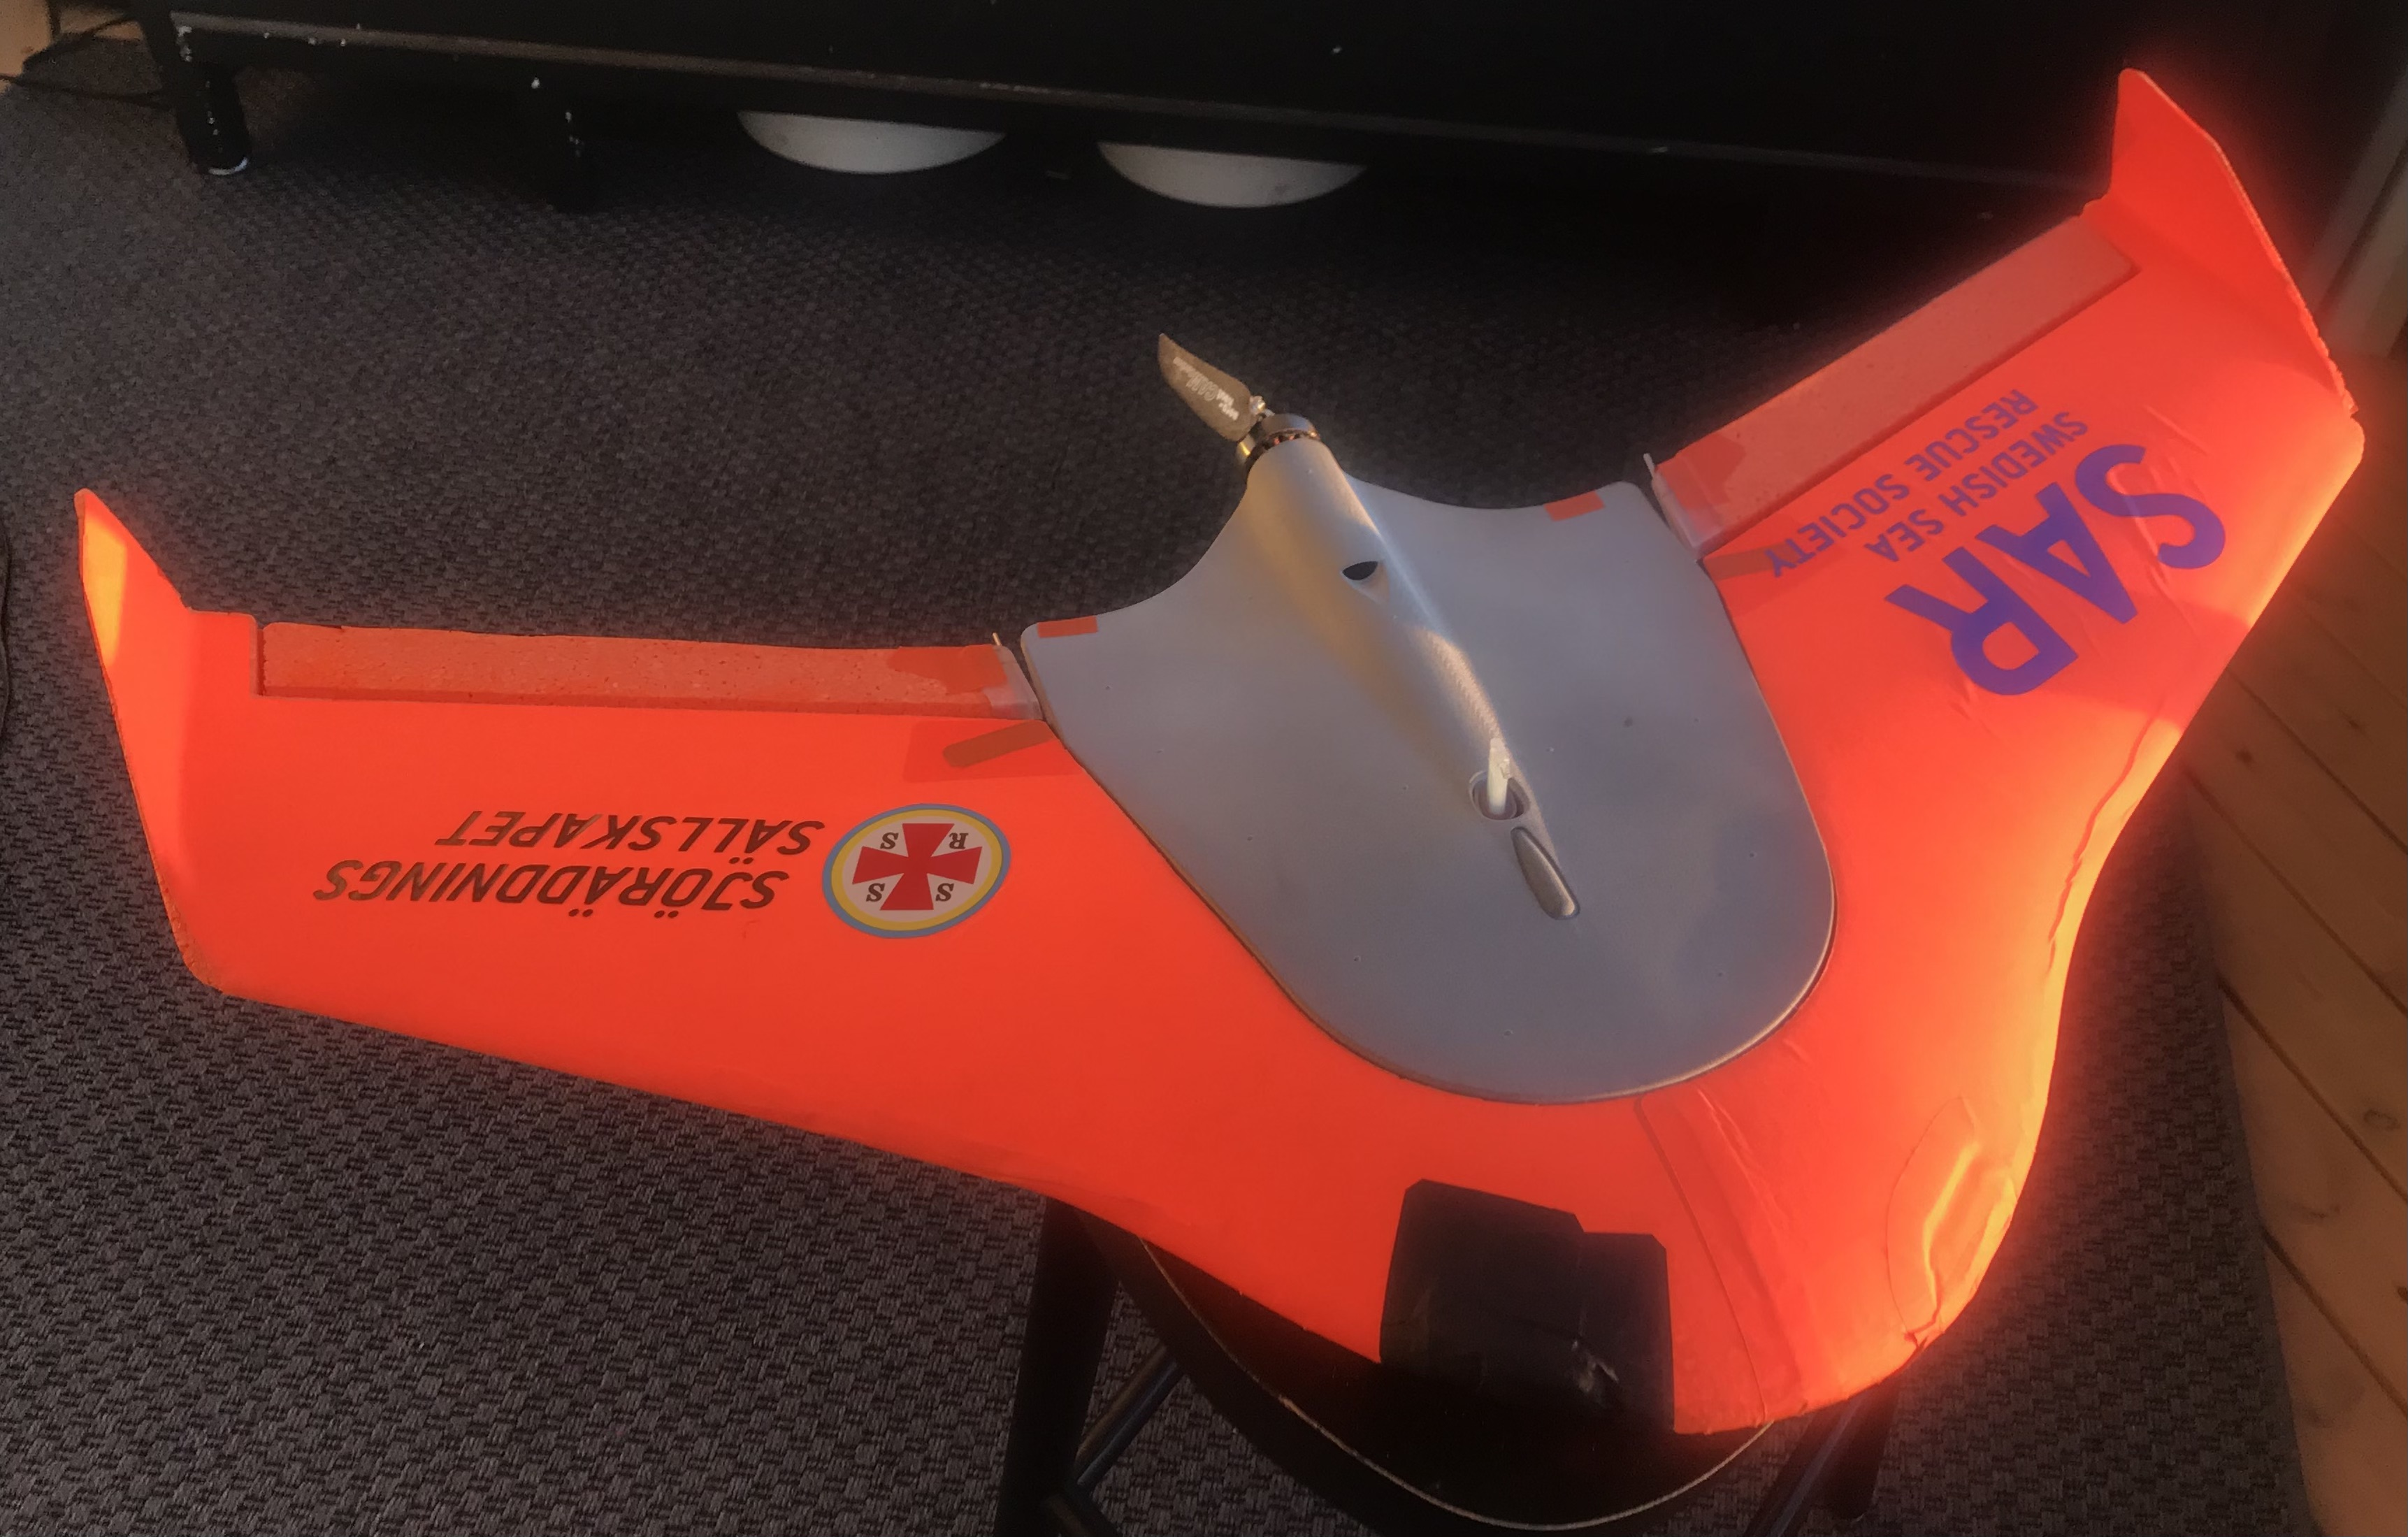
\includegraphics[width=.574\textwidth]{images/fv-3.jpg}}
   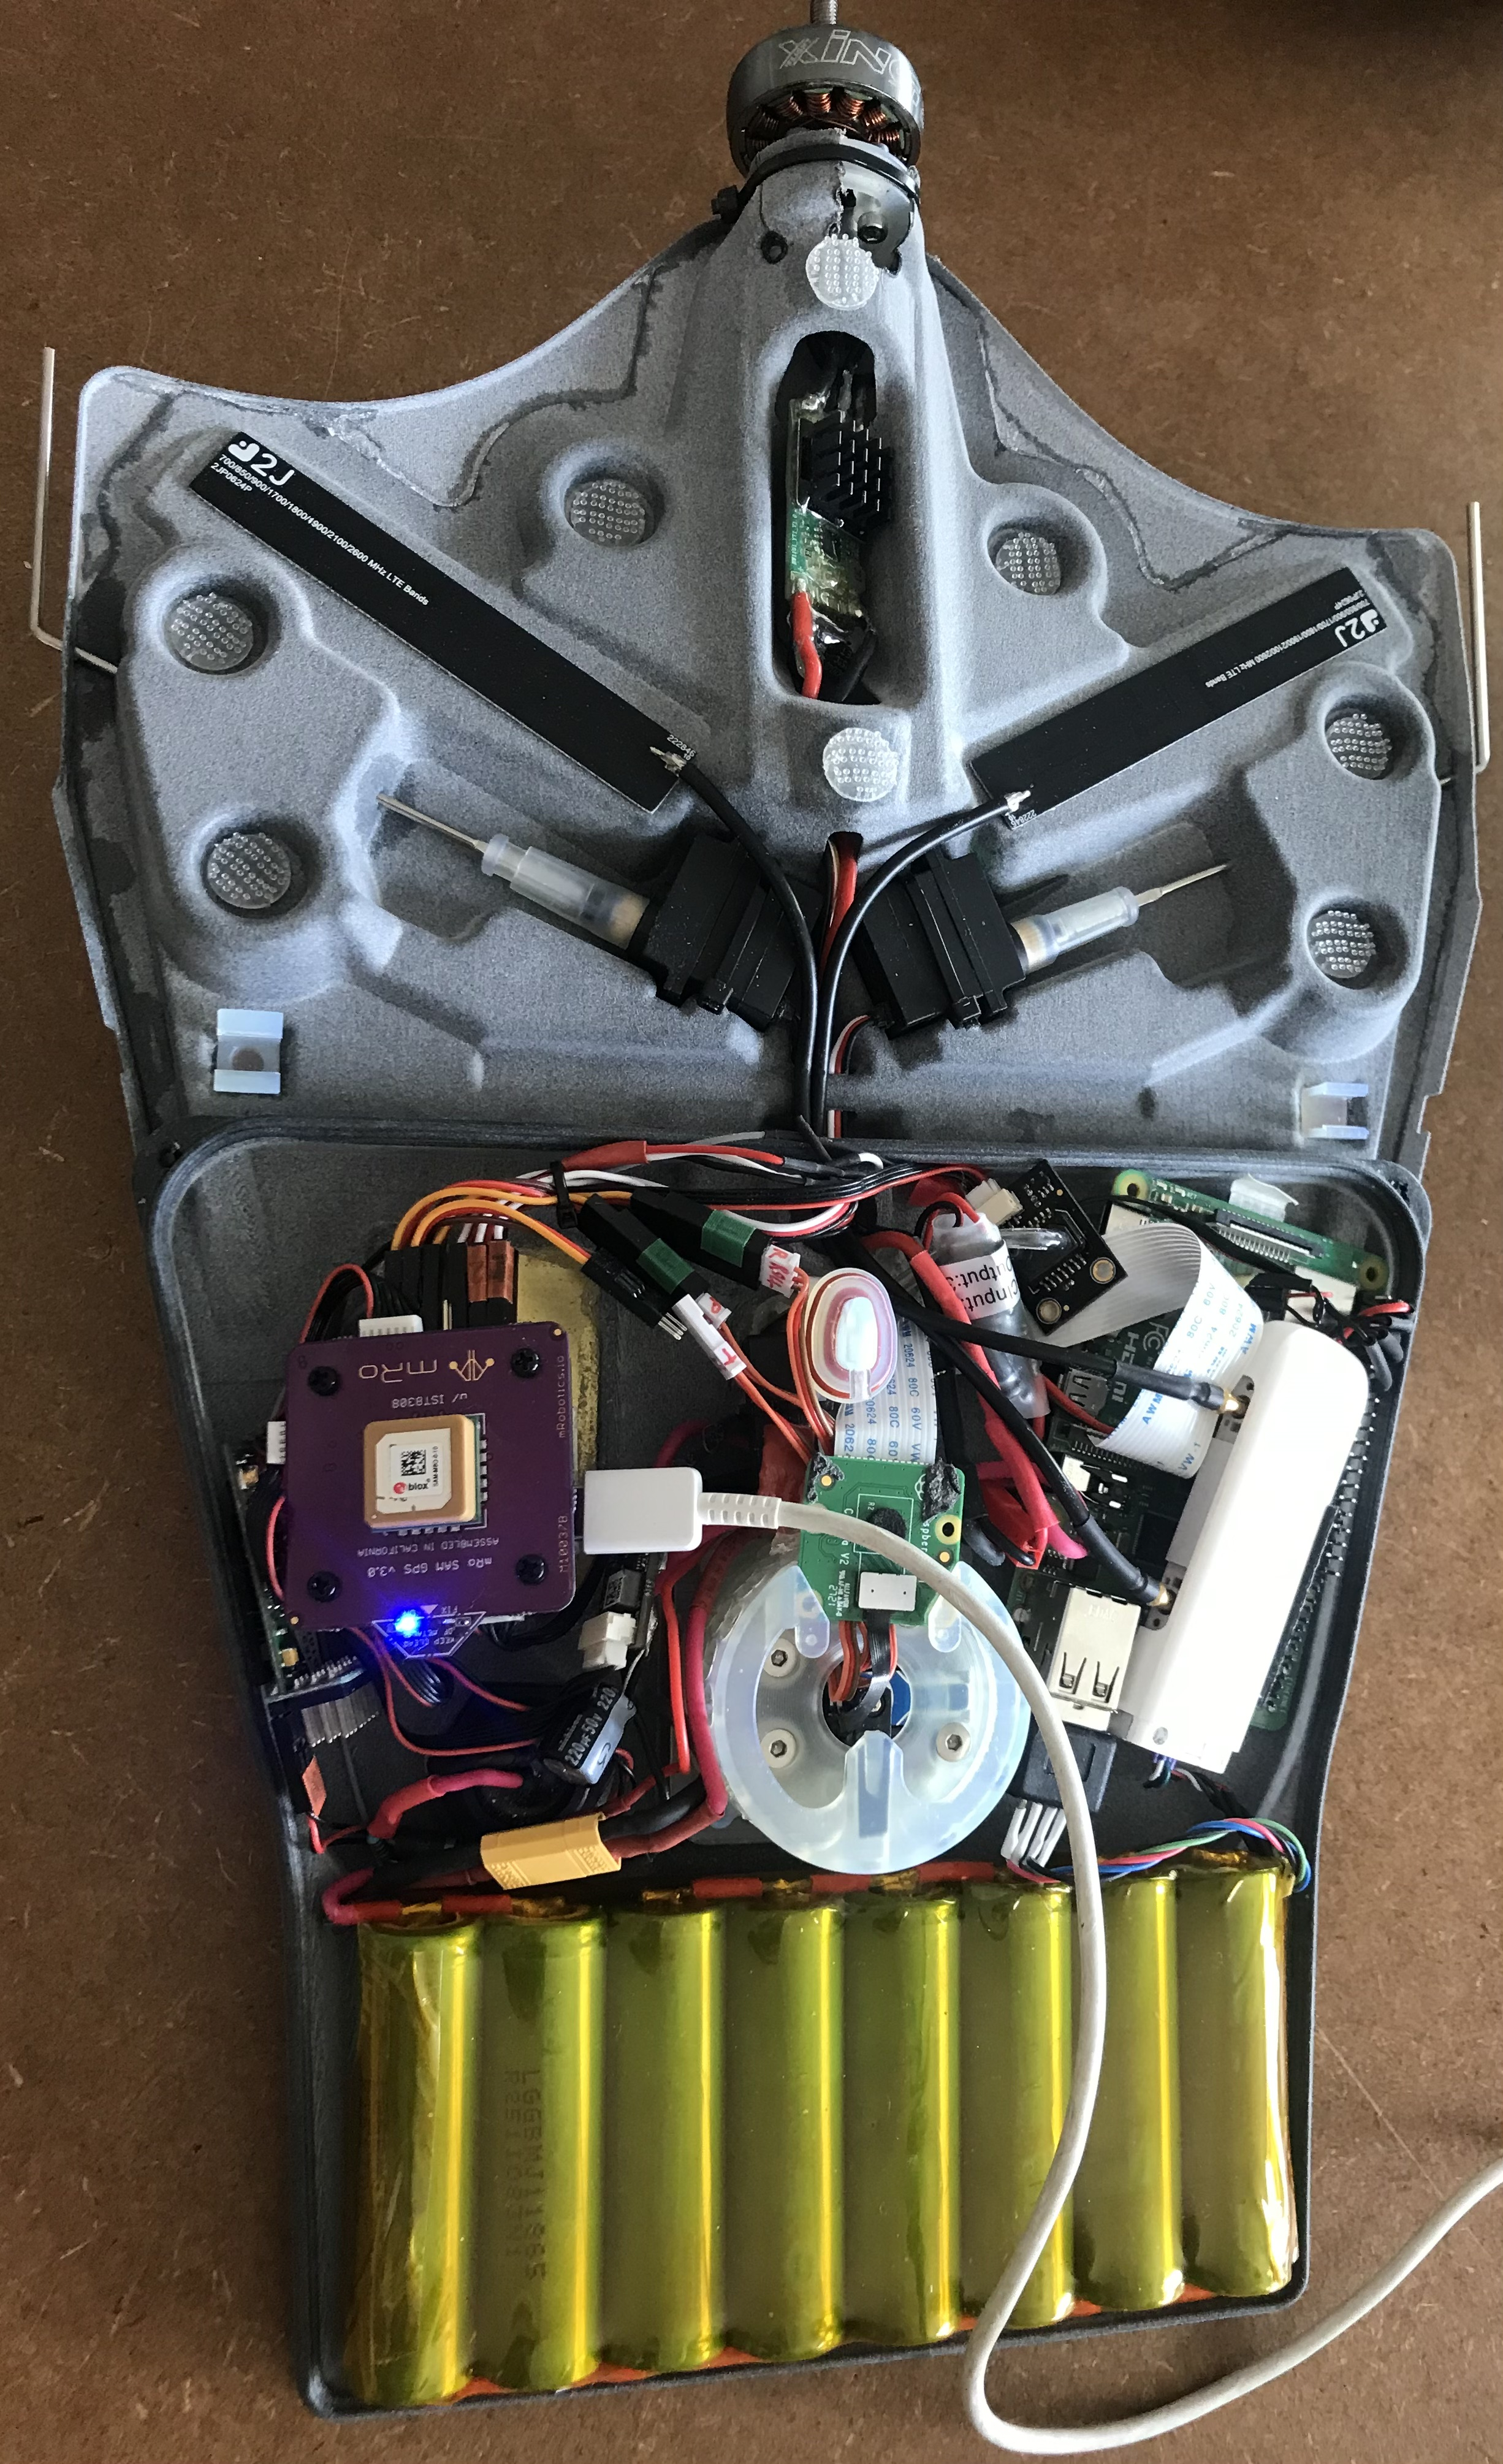
\includegraphics[width=.35\textwidth]{images/fv-1.jpg}
   \caption{The SSRS fixed-wing drone. The leftmost picture shows the full drone frame and the rightmost picture shows the inside of the drone housing with the internal components visible.}
   \label{fig:fv-drone-pics}
\end{figure}

The components relevant for this thesis work are:
\begin{description}
   \item[Flight Controller: Pixracer R15] The flight controller is the brain of the aircraft and houses components and connectors relevant to in-flight operations such as servos for control surfaces or other equipment, GPS and accelorometer.

   \item[Companion Computer: Raspberry Pi 4] The Raspberry Pi serves as the onboard computer, commonly known as the "companion computer" in the context of drone hardware. It is connected to the flight controller via USB and makes it possible to relay messages sent over ethernet instead of radio, allowing to connect to a ground station over the Internet. 
   
   \item[4G Modem] Sim-card modem allowing access to the mobile network. 
   
   \item[Raspberry Pi Camera Module v2] The camera module is a small camera that is mounted inside on a flat surface on the gimbal. The camera connects to the module board which is then connected to the Raspberry Pi with a ribbon cable. It is capable of recording 1440x1080 video at 30 fps and has a 4:3 aspect ration. 

   \item[Camera Gimbal] The camera gimbal on the drone is designed and manufactured by Fredrik Falkman at the SSRS. It is a 3D-printed design that has three degrees of freedom made possible by three servos connected to drive belts that control each axis of the camera. The servos are connected to the flight controller which also provide them with power. The gimbal is designed to house a small camera which when mounted looks out from the bottom of the drone. In \ref{fig:gimbal-pics} the schematics of the gimbal can be seen. 
   
   \begin{figure}[htp]
      \centering
      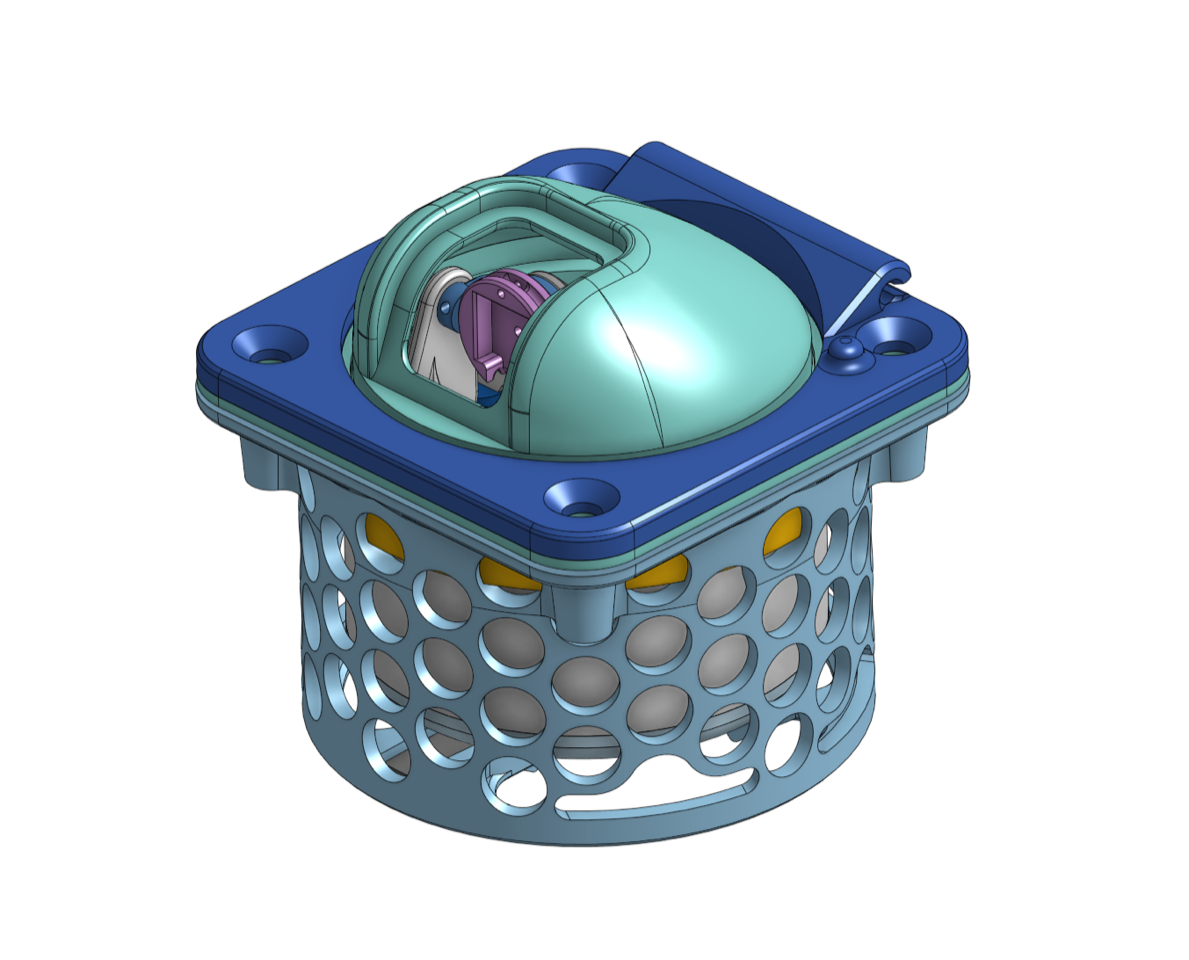
\includegraphics[width=.3\textwidth]{images/gimbal-1.png}\hfill
      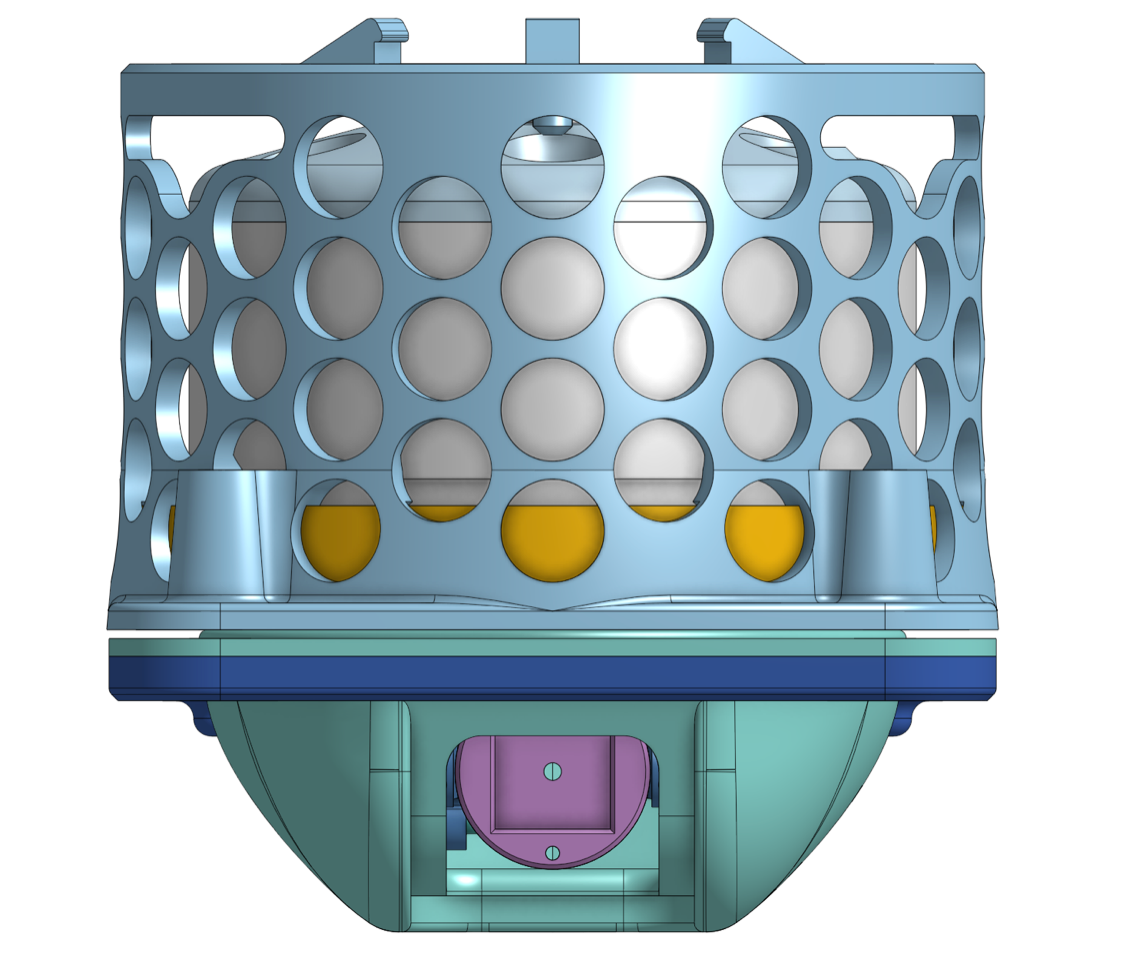
\includegraphics[width=.3\textwidth]{images/gimbal-2.png}\hfill
      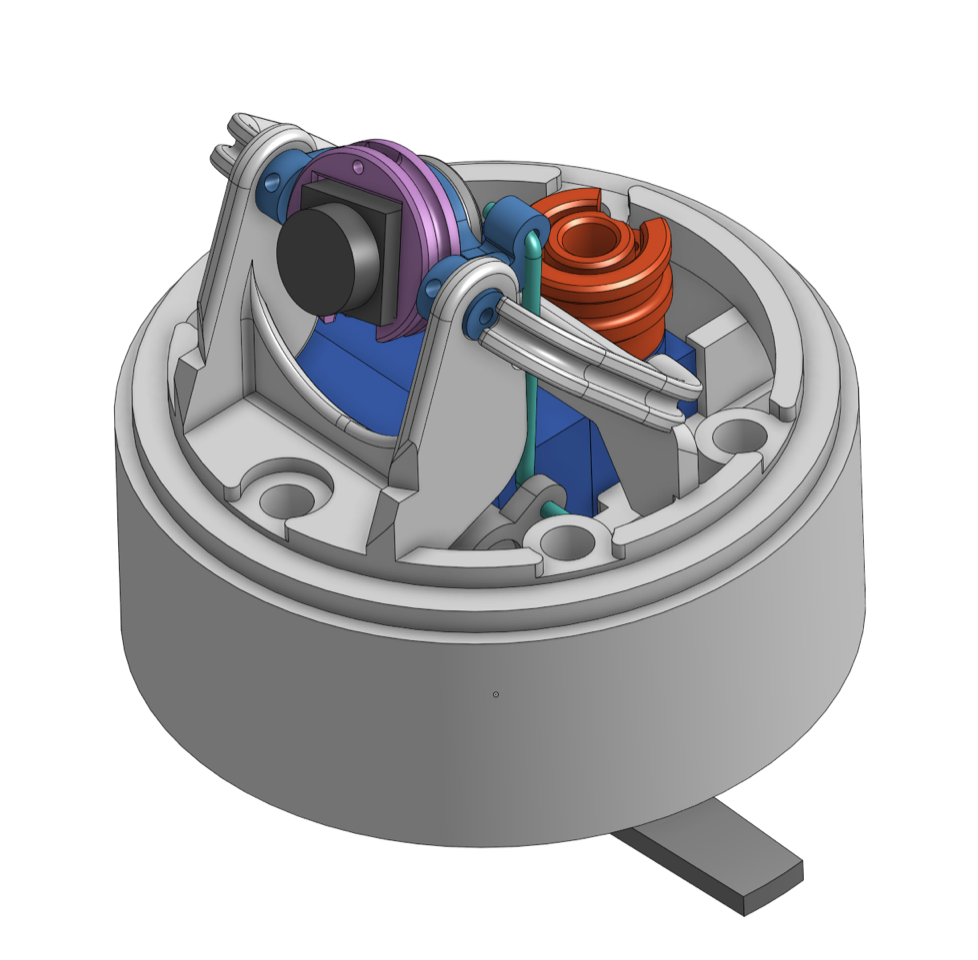
\includegraphics[width=.3\textwidth]{images/gimbal-3.png}
      \caption{Schematics of the drone gimbal. The middle and left picture shows the gimbal with its full housing. To the right the housing has has been removed and a mockup camera module has been inserted on the mounting plate.}
      \label{fig:gimbal-pics}
   \end{figure}
\end{description}
   
\subsection{Gimbal Package}
As the entire drone was not needed to conduct the QoE experiment, a Raspberry Pi, flight controller and gimbal were mounted inside a 2L Ikea SmartStore. The boards were mounted inside the box with velcro tape and the gimbal was mounted in a cutout in the bottom of the box. Pictures of the box can be seen in figure \ref{fig:drone-setup}.


\begin{figure}[htp]
   \centering
   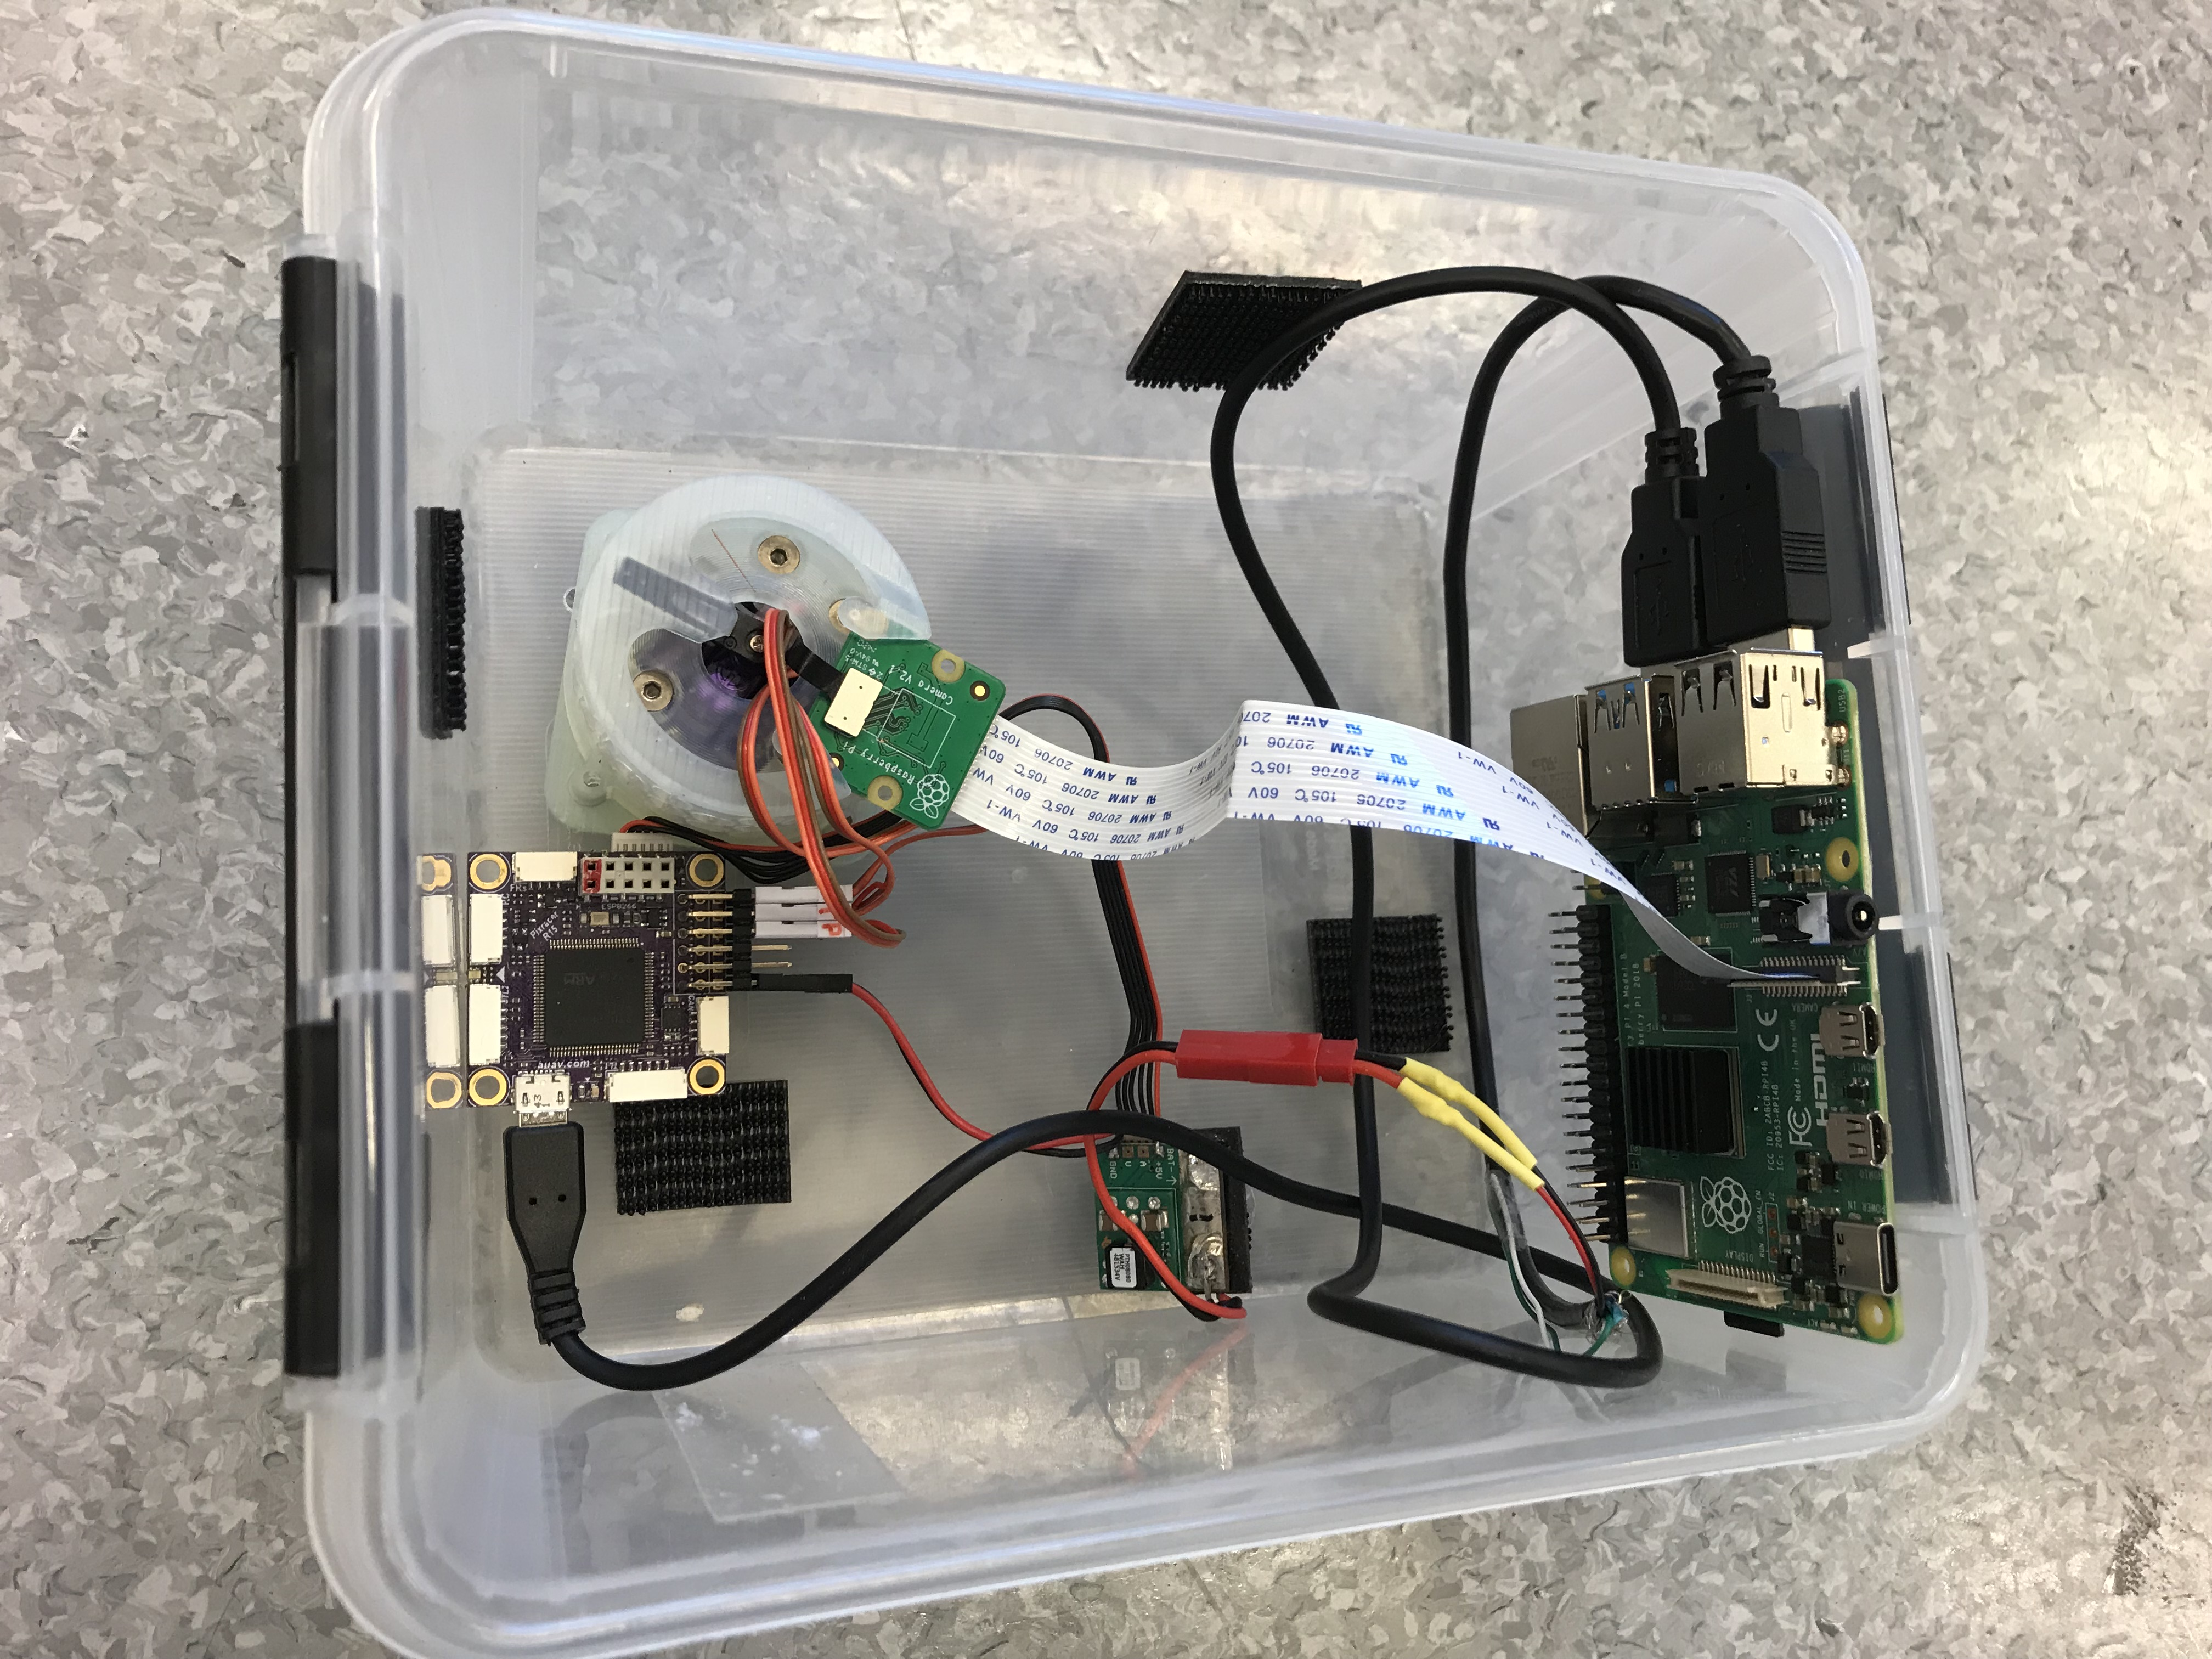
\includegraphics[width=.47\textwidth]{images/drone-box-1.jpg}\hfill
   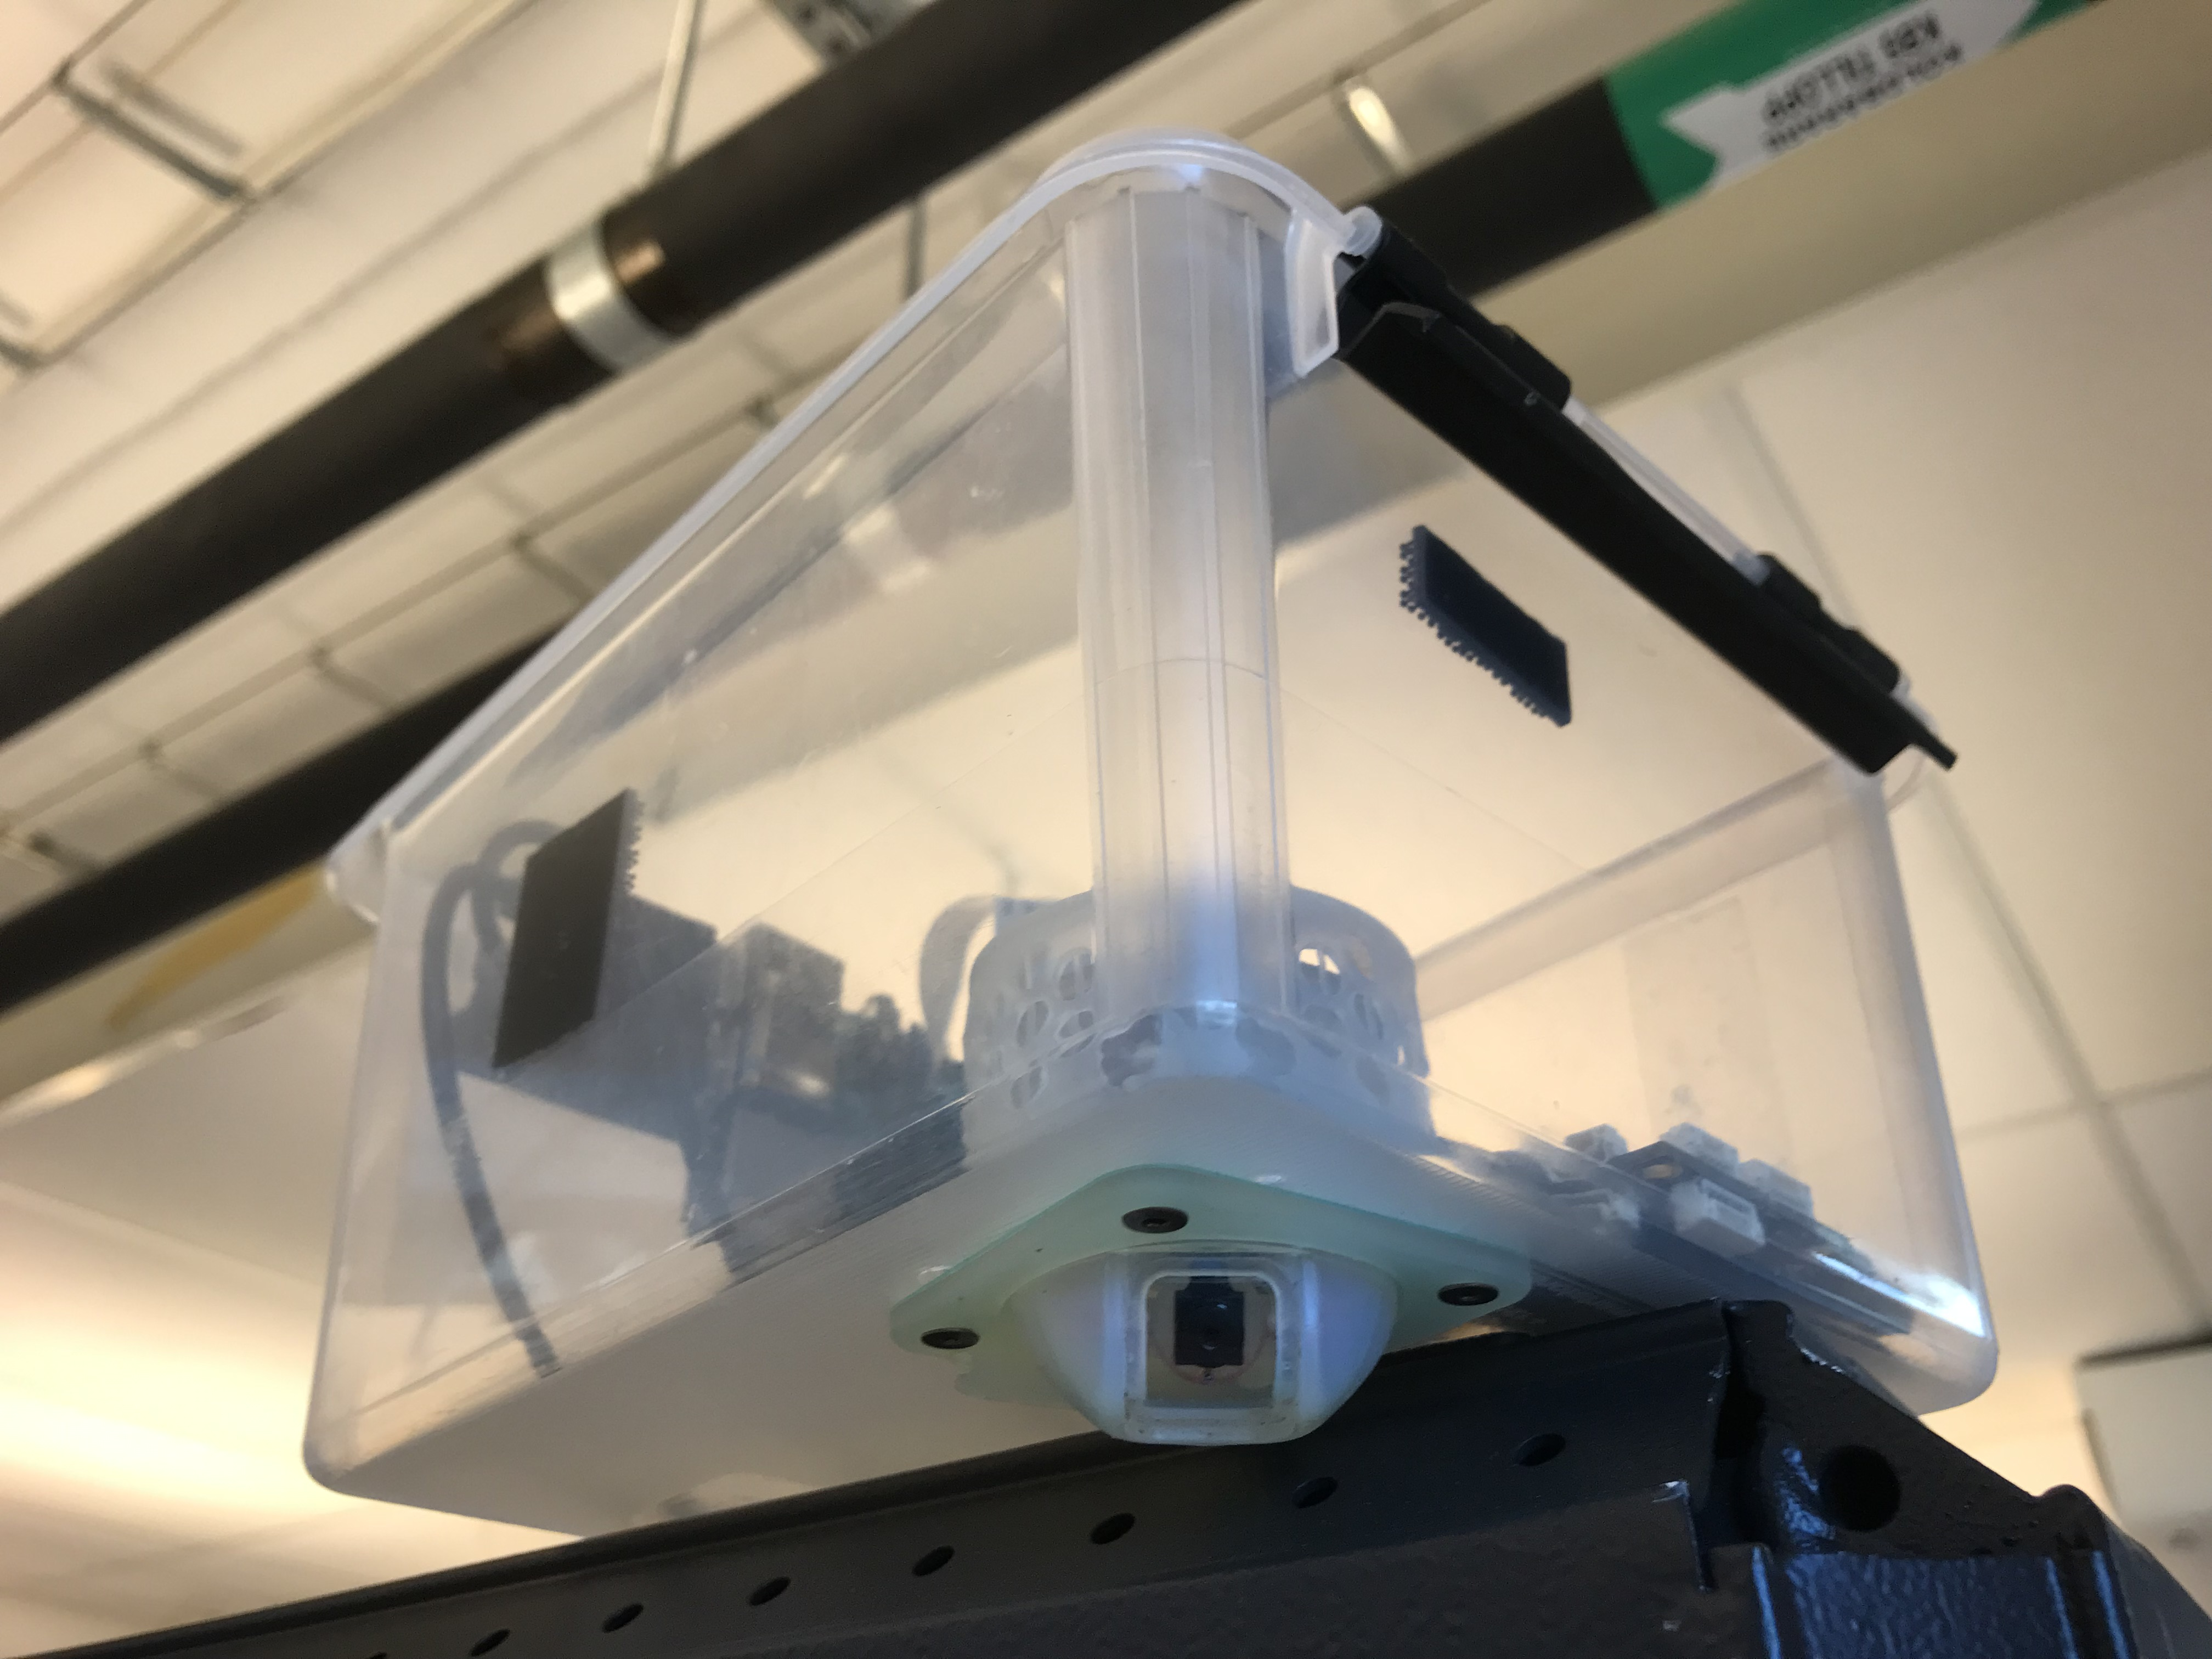
\includegraphics[width=.47\textwidth]{images/drone-box-2.jpg}
   \caption{The box that houses the drone hardware for the experiment. The left picture shows the box from above, from the left the following components are visible: flight controller, gimbal with camera module, power supply and Raspberry Pi. The right image shows the box from below.}
   \label{fig:drone-setup}
\end{figure}

\subsection{Hoverboard robot}
In order to introduce movement in the QoE experiment, a modified hoverboard was used. The hoverboard has four wheels and could be controlled via joystick inputs or coordinates. It's manouvering was assisted by real-time lidar-mapping of the room. The hoverboard can be seen in \ref{fig:hoverboard}

\begin{figure}[!hbt]
   \centering
   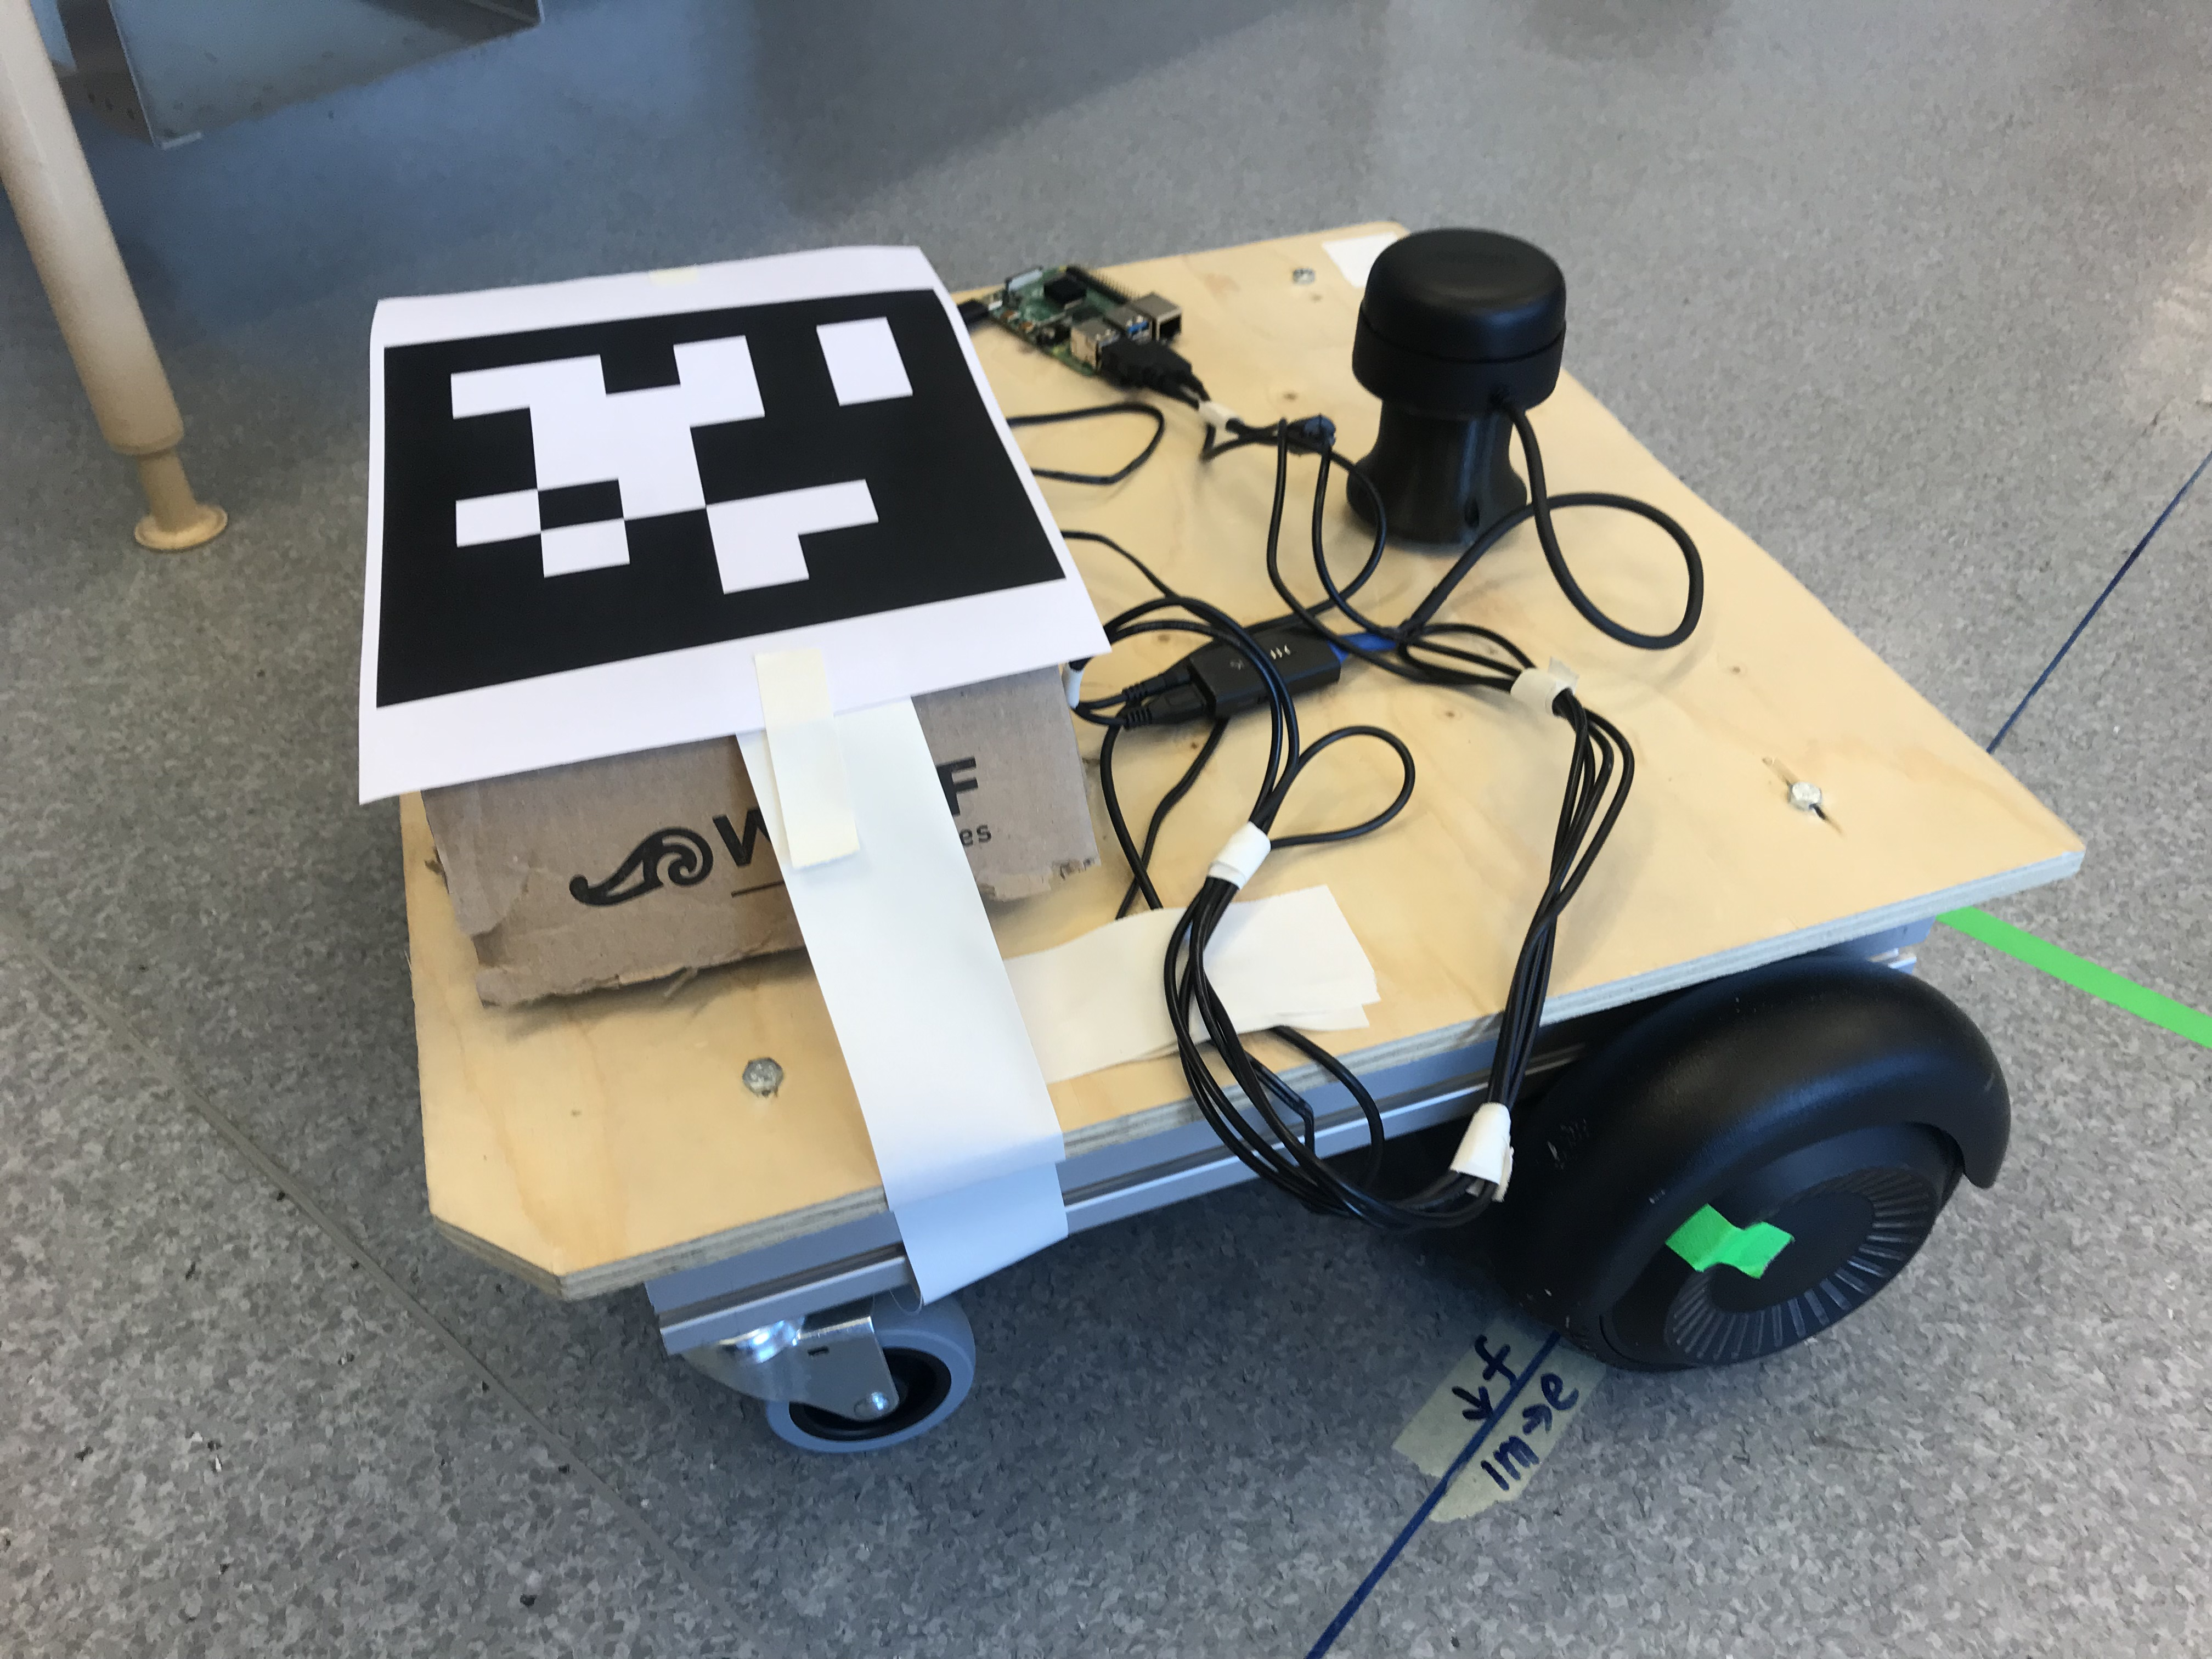
\includegraphics[scale=0.07]{images/hoverboard.jpg} 
   \caption{}
   \label{fig:hoverboard}
\end{figure}

\subsection{Apriltag}
An apriltag is a type of low-resolution QR-code often used in robotics to estimate orientation and position of robots or objects with the help of computer vision. It was fastened on top of the hoverboard as high as possible without blocking the lidar. The apriltag can be seen mounted on the hoverboard in figure \ref{fig:hoverboard}.

\section{Pre-existing Software}
In this section the software used in the experiments will be detailed.
\begin{description}
   \item[Firmware: ArduPlane]
   The firmware running on the flight controller is called ArduPlane, which is part of the open-source autopilot software suite ArduPilot that enables the creation of unmanned, autonomous vehicles \cite{ardupilot-org}. It is developed by a community of developers and is available on GitHub \cite{ardupilot-github}.
   
   \item[Protocol: MAVLink]
   As can be read on their website \cite{mavlink}, MAVLink is a lightweight protocol suited for communication with drones and between drone components. It has a byte overhead of 14 bytes and allows for concurrent communication between up to 255 systems. 

   \item [Software: MAVProxy]
   MAVProxy \cite{mavproxy} is a software running on the companion computer whose task is to relay MAVLink messages from an ethernet interface to the flight controllers serial interface. 

   \item[UV4L]
   UV4L is a video streaming server that supports several real-time communication protocols and video encodings \cite{uv4l}. It's function in the test bed is to stream the video from the camera to the web. As for video encoding, MJPEG was used.
   
   \item[Janus Server]
   As described on their webpage \cite{janus}, Janus is a plugin-based software that helps establish WebRTC connections. In this thesis it is used to establish the connection between the UV4L server and the web browser, enabling the peer-to-peer connection between the two devices.

   \item[Hoverboard software] The hoverboard has software which allows it to be controlled by a game controller or follow a set of points using coordinates for which it uses it's Lidar and a SLAM-algorithm. This makes it possible to have the hoverboard run in a programmed route with little error. 
\end{description}

\section{Gimbal Control Interface}
Using the previously described hardware and software, a program was implemented in Python displaying the video feed from the drone camera while taking control inputs from the operator. The inputs came from the joystick of a PlayStation-controller, and the program sent messages to the flight controller updating the position of the gimbal at a desired frequency and delay. The program could also record the video feed displayed to the gimbal operator. A visual overview of the system is shown in Figure \ref{fig:system-overview}.
\begin{figure}[!hbt]
   \centering
   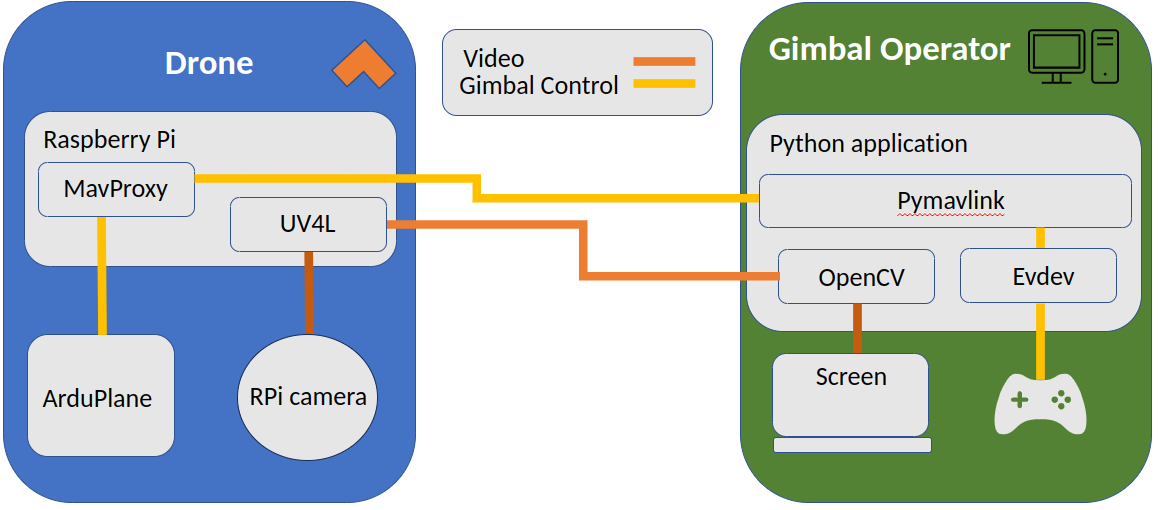
\includegraphics[scale=0.5]{images/system-overview.png} 
   \caption{An overview of the entire system. On the left, the drone and it's components including the RPi, RPi camera module and the flight controller are shown. On the right, the ground station and its' components including the web application, Janus server and the controller are shown. The colour of the connections represent what data they transfer, where orange is video, orange double-line is video negotiation and yellow is control.}
   \label{fig:system-overview}
\end{figure}

The application was run with Python version 3.9.16 and used the following libraries:
\begin{description} 
   \item [pymavlink (v. 2.4.37)]
   An interface to communicate with MAVLink devices, available at \cite{pymavlink}. With the library a port can be set to send and receive MAVLink messages.
 
   \item [Evdev v. (1.6.1)]
   A python library for interrupt-driven input devices. It is used for reading input from the Playstation-controller. Available at \cite{evdev}.

   \item [OpenCV (v. 4.7)] 
   Open Computer Vision, a very popular library for video and computer vision tasks. In the test interface it is used for displaying and recording the video feed. Available at \cite{opencv}.

   \item[Multiprocessing]
   This standard module was used in order to run the video tasks in different processes to not interfere with the control. The video frames were accessed and displayed by one process and then feeded to another process saving each frame. For more information on the library see \cite{multiprocessing}.  
\end{description}

Delay in the controls could be introduced by providing a program argument. The delay was simulated by putting each outgoing message in a queue along with a timestamp, with the program waiting until \ timestamp + delay \ was reached before sending the command. The following algorithm was used to schedule the sending of commands according to the delay:
\begin{algorithmic}
   \While{running}
   \State $timestamp, pitch, yaw = queue.get()$ // blocking call
   \State $t_{0} = time.now$
   \State $diff = timestamp + delay - t_{0}$
   \If{diff > 0}
      \State $time.sleep(diff)$
   \EndIf
   \State $send\_command(pitch, yaw)$
   \EndWhile
\end{algorithmic}

The screen and the controller were then filmed on a phone in 120 FPS to measure the time between a control input to the video feed updating. To measure the network delay a simple ping-measure was taken.

The network latency was found to be below 1 ms. The delay of the video feed alone was between 100-150ms while the full controller to video feedback delay was around 400ms. 

\subsection{Sources of Delay}
Although the sources of the delay were not examined in any further depth there were a some known sources of the delay:
\begin{description}
   \item[Message frequency] 
   While the internal model of the gimbal's orientation was updated by interrupts, the message rate to the flight controller was set to a maximum of 20Hz, resulting in a delay between 0-50ms.
   
   \item [Video encoding]
   The delay of the video feed was measured by recording a stopwatch, the controller and the video feed of the stopwatch simultaneously. The difference between the stopwatch on the recording and the screen was estimated to be between 100-150ms.
   
   \item [Network delay] 
   The network delay was measured with pings to be below 1ms. 

   \item[MAVProxy relaying] Each message must be taken from the ethernet interface of the Raspberry Pi and be sent on the serial interface to the flight controller. An estimate of this time was not made.
   
   \item[Flight Controller] The flight controller must process the message and send the appropriate PWM signals to the gimbal motors. The processor running the firmware is a small chip and it is possible that gimbal control is not a high priority message in the software. An estimate of this time was not made.
\end{description}

\subsection{Design Choices} 
This section aims to explain some of the design choices that were taken during development of the gimbal interface. It can be skipped if the reader is not interested in the development process.

\subsubsection{Video streaming}
In the real drone system the video feed is done with WebRTC. This is a modern peer-to-peer video protocol well suited for the application of video from IoT, and the intention was to use this in the test bed as it had a low latency and was accessible through the browser. The goal was to get the raw video feed to OpenCV in order to adjust image parameters as well as for detection and recording of the images. Unfortunately, the raw video feed proved difficult to access as other video processing software had to be used along with the peer-to-peer negotiation. In the end the MJPEG format was chosen, as it had acceptable delay and could be integrated only by providing a HTTP source to the OpenCV video capture module.

\subsubsection{Native vs. web}
The application that the SSRS currently use for mission control is hosted on the web, and as such the test bed was initially developed as web-application. This proved difficult for the developer as they had limited experienced working with web applications. As the amount of tasks for the program to perform grew, a decision was made to implement the test bed as a native Python application instead. This made it easier to orchestrate the video and control tasks using regular UNIX processes from the Python multiprocessing library. 

With this decision the possibility to remotely host the application was lost, but as the goal was to develop a working test bed this was deemed acceptable. 

\section{Result Script}
\label{sec:resultscript}
In order to extract the results from the recorded video, a Python-script running the detection algorithm was implemented. 

The script used the following python libraries:
\begin{description}
   \item[OpenCV] Video tasks and image processing.
   \item[dt-apriltags] Detection algorithm.
   \item[math] Mathematical operations, such as calculating the distance between two points.
   \item[sys] Iterating over directories, reading and writing files.  
\end{description}

Pythagoras' theroem was used for calculating the pixel distance between the two points and is shown in equation \ref{eq:distance}. A frame from the detection script can be seen in figure \ref{fig:resultcalc}.

\begin{equation}
   \label{eq:distance}
   \overrightarrow{px} = \sqrt{(x_{hoverboard} - x_{center})^2 + (y_{hoverboard} - y_{center})^2}
\end{equation}


\begin{figure}[!hbt]
   \centering
   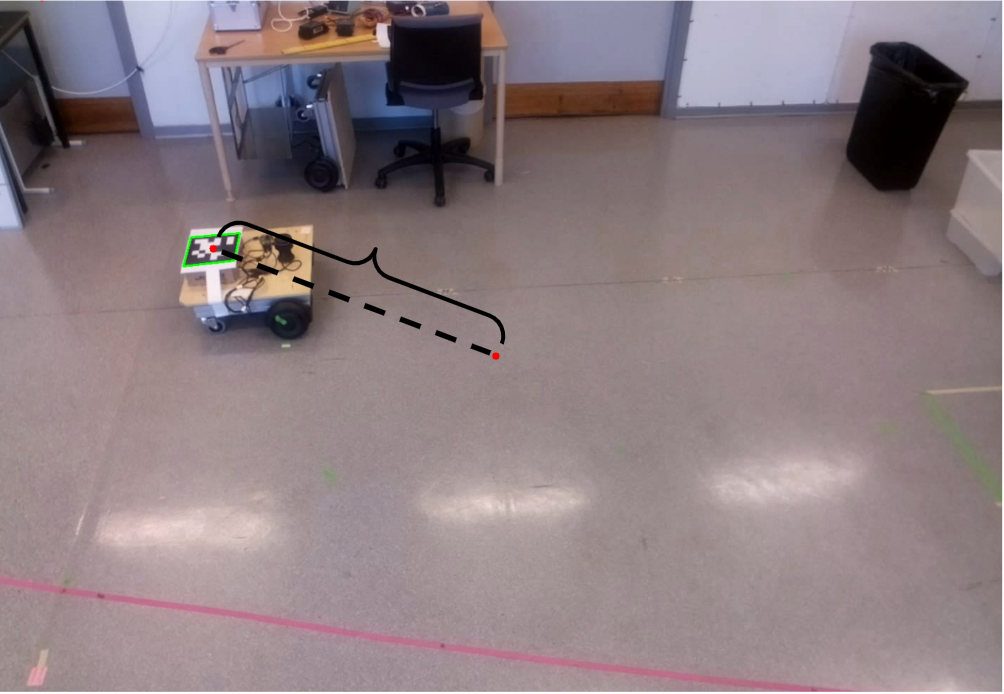
\includegraphics[scale=0.3]{images/resultcalc.png} 
   \caption{Example of a result from the detection algorithm. The green square outlines the result of the detected object and the red dot its' center. The error is the distance between the two dots as outlined by the black indicators.}
   \label{fig:resultcalc}
\end{figure}

The script took each frame of a recorded trial and ran the detection algorithm on it. If an apriltag was detected in the image, the distance between the center of the apriltag and the center of the screen was saved with the corresponding frame number in a CSV-file named after the subject and the specific trial. In case of no detection, a NaN value was inserted for that frame. The video with the detection overlay was also saved for later inspection.

\section{Auto-follow mode}
As a proof of concept, an auto-follow mode was developed which allowed the gimbal to follow the apriltag. This was made using the object detection algorithm from the result script coupled with a PI-controller which had the center of the image center as reference value. Due to time limitations this was not investigated any further.

\chapter{Experiments}
This chapter will describe the setup, procedure and evaluation of the two experiments that were performed.

\section{QoE Lab Experiment}
This section describes the procedure of the experiment aimed at evaluating the effect of latency on the gimbal operator using the hoverboard robot. 

\subsection{Task}
The task was to keep the center of the screen, marked with a red dot (as seen in \ref{fig:interface}), aligned with the center of the apriltag laying on top of the hoverboard (shown in \ref{fig:hoverboard}) while moving in an elipse.

\subsection{Experimental Setup}
The experiment was set up in a lab where the subject and the conductor sits at a desk with a high shelf behind them obscuring the view towards the rest of the lab. Behind the shelf the robots used in the experiment are located. An illustration of the lab setup is provided in figure \ref{fig:exp-setup}. 

\begin{figure}[!hbt]
   \centering
   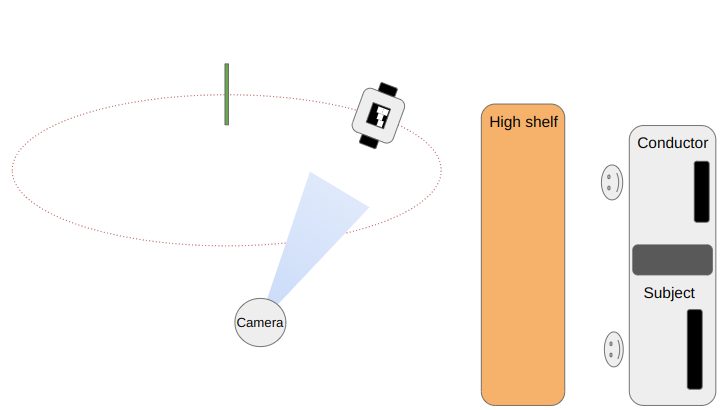
\includegraphics[scale=0.3]{images/exp-setup.png} 
   \caption{An overview of the experimental setup. To the right the experiment conductor and subject by a desk facing right. On the left side, behind the shelf, the test bed including the camera and the hoverboard are located. The camera is mounted at a height of 2.1 meters with the gimbal facing down.}
   \label{fig:exp-setup}
\end{figure}

An image of the hoverboard and the camera is shown in image \ref{fig:real-exp}.

\begin{figure}[!hbt]
   \centering
   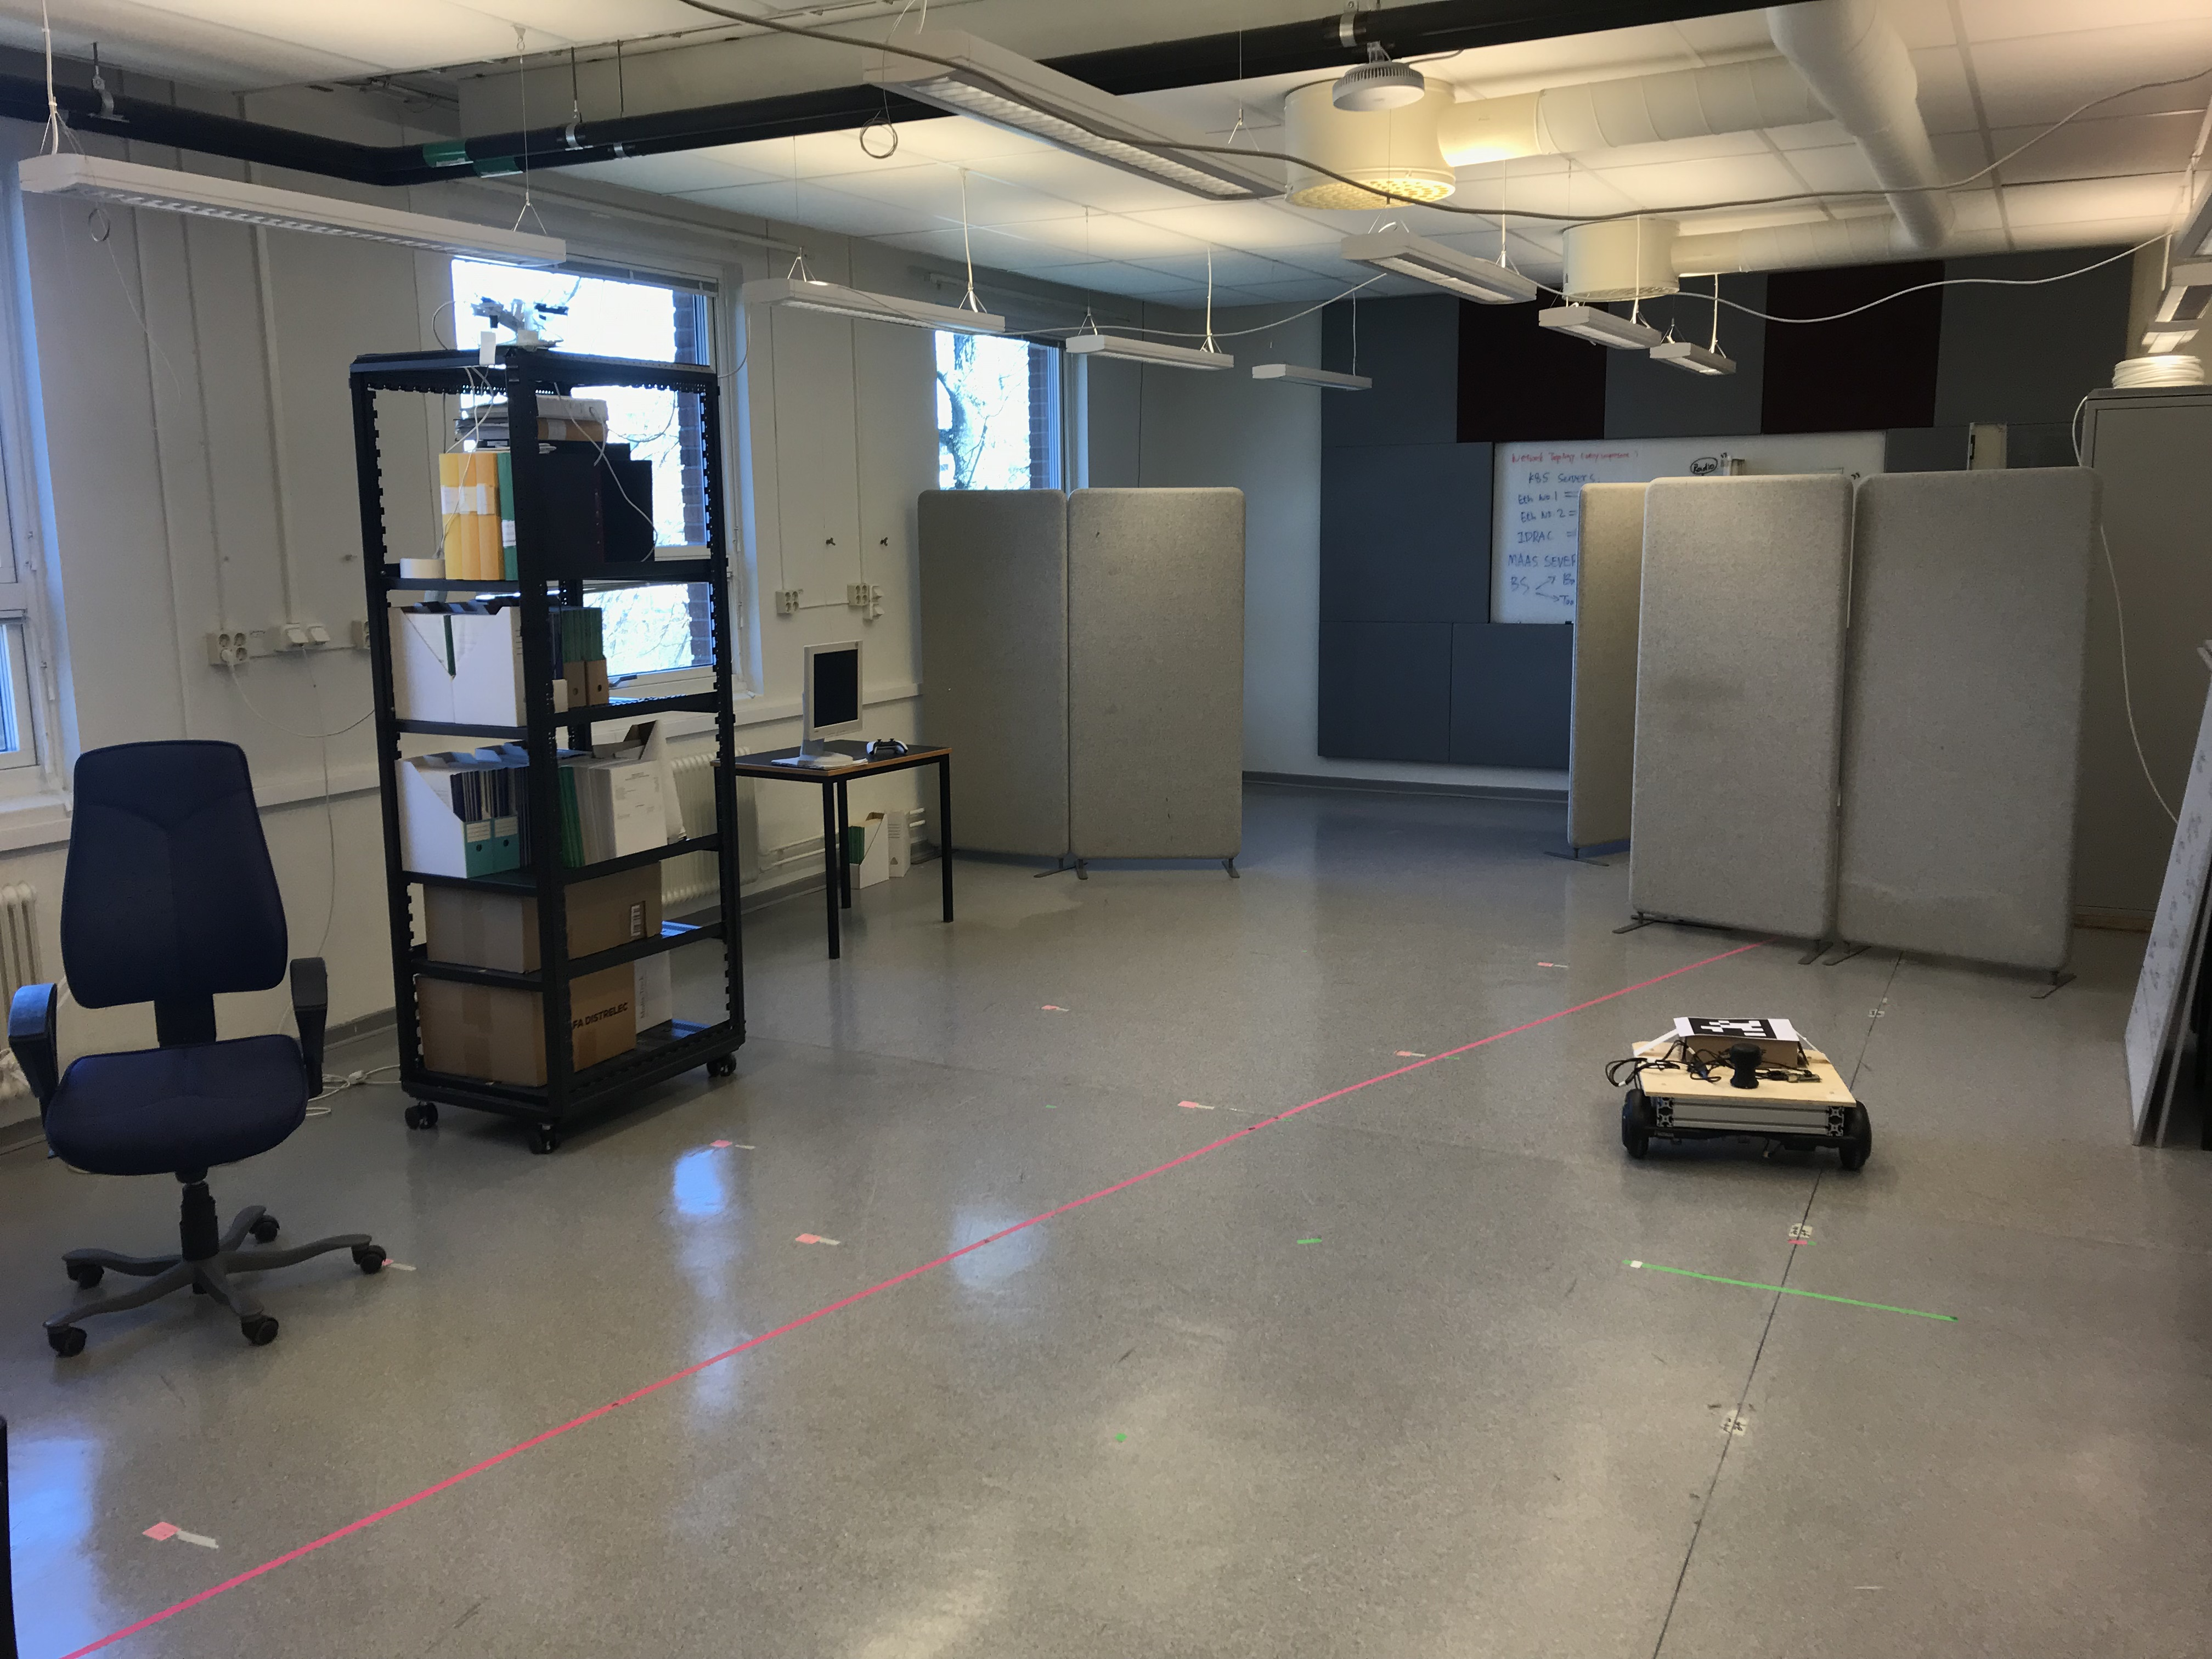
\includegraphics[scale=0.1]{images/testbed.jpg} 
   \caption{A picture of the test bed. On the left side there is a server rack with the drone box mounted on top. The hoverboard can be seen on the right side of the picture.}
   \label{fig:real-exp}
\end{figure}

\subsubsection{Subject selection and recruitment}
The subjects were recruited mostly from the conductor's network of contacts, as in order for the subjects to be covered by insurance during the experiment, the subjects had to be either be students or employed by Lund University. Some of the participants came spontaneously while others booked a time in a spreadsheet provided by the conductor.

There were 10 test subjects, 4 women and 6 men, with an average age of 26.1 years where the youngest was 23 and the oldest 37. Furthermore, they were questioned about their eyesight, handedness as well as experience with FPV-games and flying drones.

There was no compensation for the subjects other than home baked goods and a hot beverage, which were offered at the beginning of each experiment. 

\subsubsection{Lab Conditions}
The lab is located in the E-building at LTH, Lund University. It can also be mentioned that the windows in the room face north, so there was no risk of direct sunlight during the experiments.
The computer screen was 24' and the application was run on a machine with the following specifications:
\begin{description}
   \item[CPU] Intel Core i7-4770 @ 3.40GHz, 4 cores 8 threads
   \item[RAM] 16 GB
   \item[GPU] Mesa Intel HD Graphics 4600 (HSW GT2)
\end{description}

\subsection{Experimental Procedure}
In this section each of the steps will be described in more detail. The experimental procedure is summarized in the table \ref{tab:task-timeline}.

\begin{table}[ht]
   \centering
   \caption{Task Timeline}
   \label{tab:task-timeline}
   \begin{tabular}{|c|l|l|}
   \hline
   \textbf{Time (approx.)} & \textbf{Task} & \textbf{Instruction} \\ \hline
   3 & Coffee and cookies & \\ \hline
   5 & Introduction & Tell the subject about what the study is about. \\
   & & Gather personal data + consent \\ \hline
   2 & SSQ & \\ \hline
   3 & Experiment walkthrough & What is going to happen \\
   & & Description of task \\
   & & Where to aim exactly on the apriltag \\ \hline
   2 & Warm-up & The subject gets to try the setup for one lap \\ \hline
   10 & Tests & 5 tests with added latencies [0, 200, 300, 400, 500] \\ 
   & & in random order \\ \hline
   2 & SSQ & \\ \hline
   3 & Interview & \\ \hline
   30 & Total & \\ \hline
   \end{tabular}
\end{table}

\subsubsection{Introduction}
The experiment starts with the subject being seated at the desk to read through the consent form. After this was signed the conductor clarified that the subject was free to ask any question during the experiment and could choose to interrupt it without declaring any reason. 

Then, the subject fill out the background information form where they also get to choose a four digit code which from that point is the only identifier of the subject and it's results. If the subject booked a time slot in the spreadsheet, they were at this point removed from it.

\subsubsection{Experiment Walkthrough}
The task was explained to the subject while a printed apriltag with a cross on it was shown, marking the spot where to aim on the tag. The particular apriltag printed for this experiment had two white and two black squares meeting in the middle, making the center easier to identify. The apriltag shown to the subject is shown in figure \ref{fig:apriltag}.

\begin{figure}[!hbt]
   \centering
   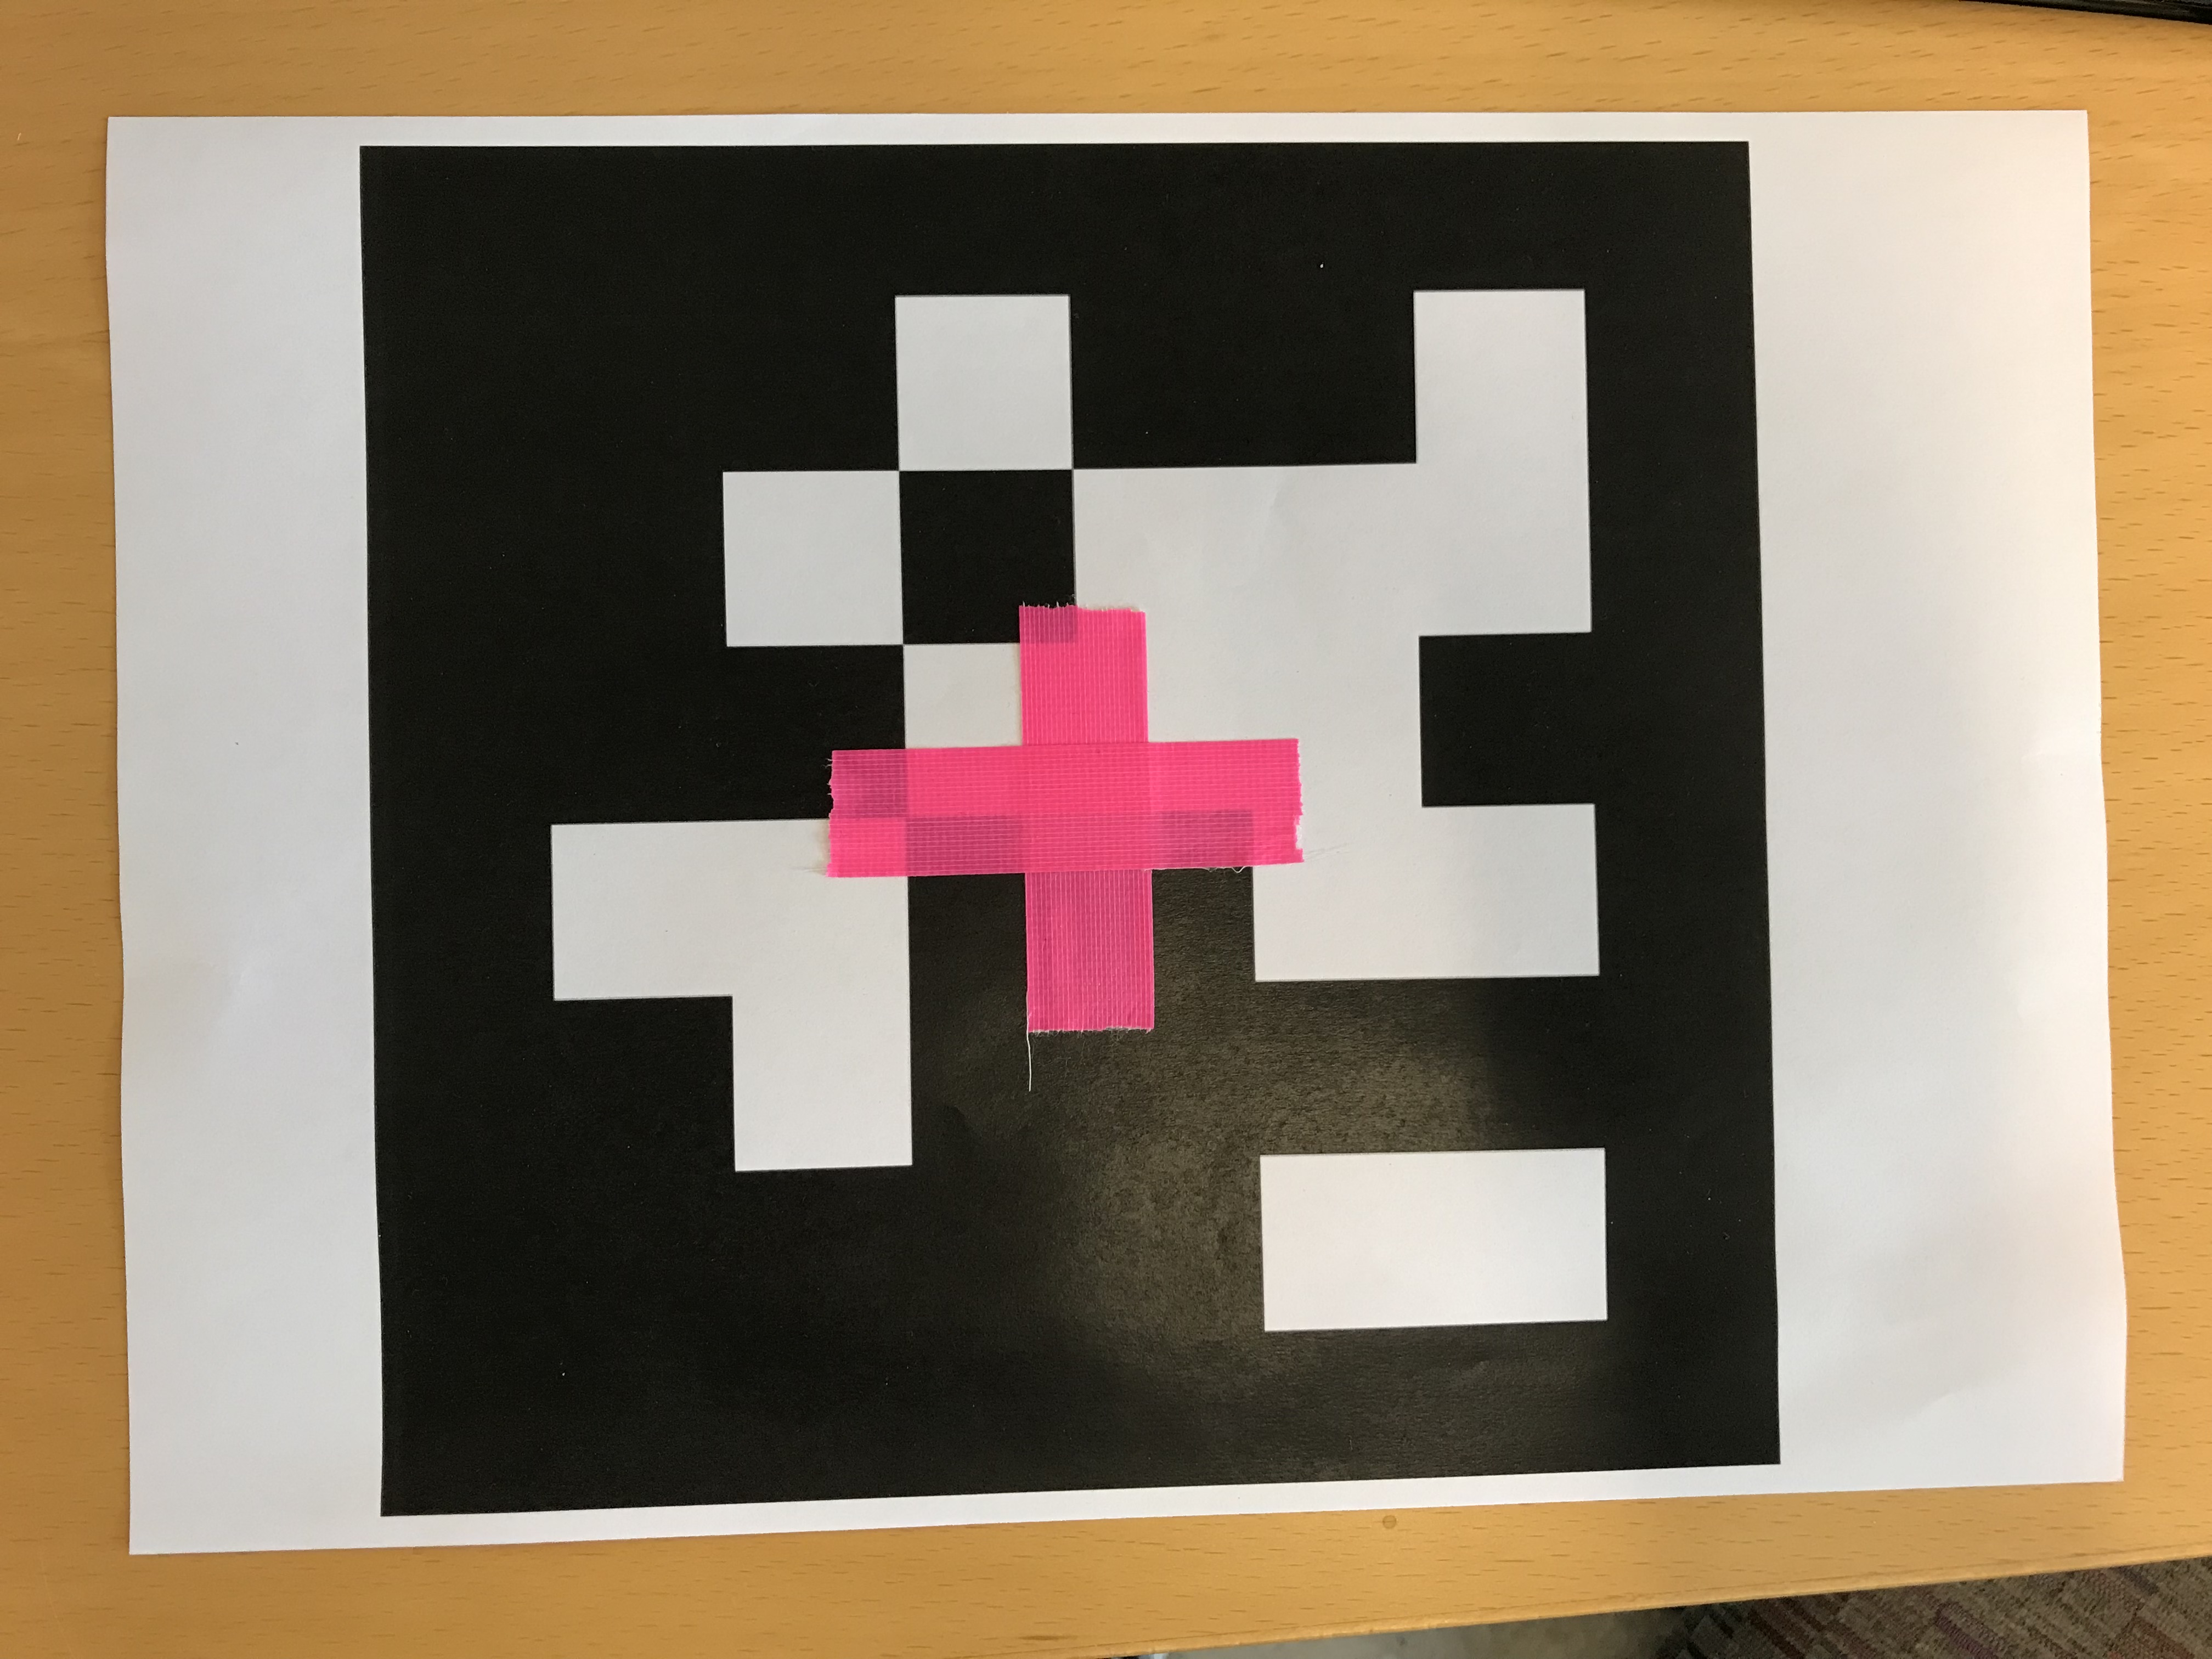
\includegraphics[scale=0.08]{images/apriltag.jpg} 
   \caption{The apriltag used to show the subject where to aim.}
   \label{fig:apriltag}
\end{figure}

The subject was then given a chance to try the system without any delay, and was given the controller and presented with the view, shown in figure \ref{fig:interface}. The hoverboard was started and ran for one lap in the same path that it would run during the test and the subject could try and follow it.

\begin{figure}[!hbt]
   \centering
   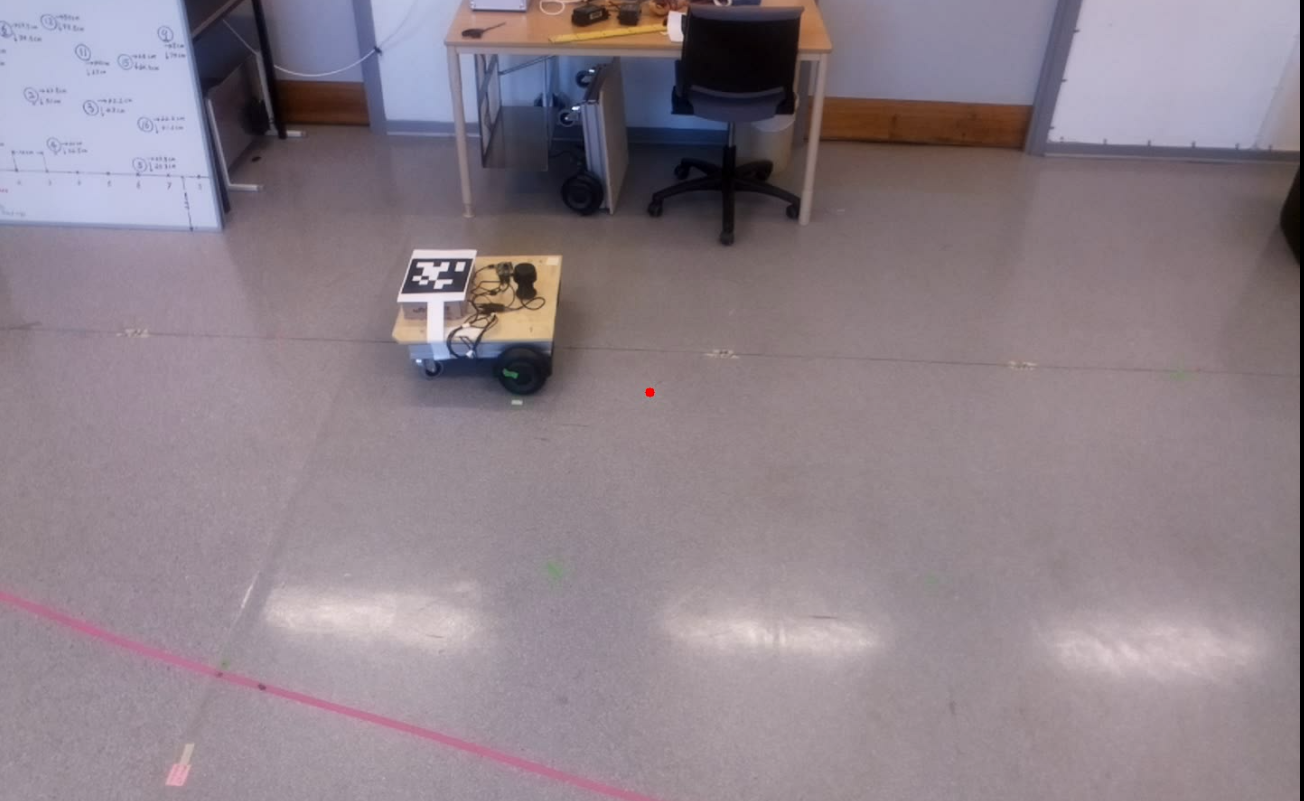
\includegraphics[scale=0.3]{images/interface.png} 
   \caption{The interface that the subject was presented with. The red dot in the middle of the screen is overlayed on top of the displayed video so that the subject has a better reference of the center of the screen.}
   \label{fig:interface}
\end{figure}

\subsubsection{Test Procedure}
After the task description and warm-up the tests commenced. The added latencies tested were 0, 200, 300, 400 and 600 and the order in which they were given to the subject was random. 
At the beginning of each trial the interface was restarted with one of the latencies induced in the system. The subject was then asked to put the red marker in the middle of the screen in the middle of the apriltag. When the subject confirmed that they were ready to start the conductor started the hoverboard. The subject followed the hoverboard for two laps, which took about 2 minutes in total.

After the laps were completed the interface was shut down and the subject was asked to rate the system by answering four different questions on a scale from 1 to 5. When the subject had answered the questions the next trial was started.

At the end of the fifth and last trial the subject got to fill in the sickness questionnaire was also asked a few interview questions by the conductor.

\subsection{Evaluation}
The following two sections will describe the quantative and qualitative methods that were used to evaluate the system.

\subsubsection{Quantative Evaluation}
To measure the performance of each subject, the result script described in section \ref{sec:resultscript} was used. This resulted in one CSV-file with about 2700 rows of data per trial. The start and end frames where extracted manually from the video of each trial and were saved in a separate file.  

\subsubsection{Qualitative Evaluation}
After each trial the subject answered a form with four questions about the system on a five degree scale, labeled 'Terrible' to 'Excellent'. The questions are shown in table \ref{tab:form-questions}. 

\setlength{\extrarowheight}{5pt}
\vspace{10pt}

\begin{table}[!hbt]
   \centering
   \begin{tabular}{|c|}
      \hline
      \textbf{How would you describe the controllability of the system?} \\
      \\
      Terrible \hspace{10pt} Poor \hspace{10pt} Fair \hspace{10pt} Good \hspace{10pt} Excellent \\    
      \\
      \hline
      \textbf{How would you rate your ability to perform the task?} \\
      \\
      Terrible \hspace{10pt} Poor \hspace{10pt} Fair \hspace{10pt} Good \hspace{10pt} Excellent \\    
      \\
      \hline
      \textbf{How pleasant was the system to use?} \\
      \\
      Terrible \hspace{10pt} Poor \hspace{10pt} Fair \hspace{10pt} Good \hspace{10pt} Excellent \\    
      \\
      \hline
      \textbf{How would you rate your impression of the system as a whole?} \\
      \\
      Terrible \hspace{10pt} Poor \hspace{10pt} Fair \hspace{10pt} Good \hspace{10pt} Excellent \\    
      \\
      \hline
   \end{tabular}
   \caption{The questions asked for each delay after each trial.}
   \label{tab:form-questions}
\end{table}

\vspace{10pt}

Right after the last trial the subject filled out the SSQ once more. Then, a brief interview was conducted with questions about the system and experience in general. The questions can be seen in table \ref{tab:interview-questions}.

\setlength{\extrarowheight}{5pt}
\vspace{10pt}

\begin{table}[!hbt]
   \centering
      \begin{tabular}{|c|}
         \hline
         \textbf{1. What was your general experience of controlling the camera?} \\
         \hline
         \textbf{2. Did you experience any difference in the controls between the trials?} \\
         \hline
         \textbf{3. Was there any part of the track that was harder than any other?} \\
         \hline
         \textbf{4. Do you think the system would have been usable with the worst experimental conditions?} \\
         \hline
         \textbf{5. Do you think training would have helped an operator get better using the system?} \\
         \hline
      \end{tabular}
   \caption{The interview questions asked by the conductor after the last trial.}
   \label{tab:interview-questions}
\end{table}

\vspace{10pt}


\subsection{Known Sources of Error}

\subsubsection{Ecological validity}
The future operators of the system are to be the volunteers of SSRS, which have a wide variety in age and background. Thus,there are three main concerns with the ecological validity of the study. Firstly, the subjects were all either students or researchers at Lund University. Secondly, the average age of the subjects was low. Lastly, the sample size was only ten people. 

The last concern is probably least important when it comes to the validity of the study, as the low number of participants could be compensated for by having each subject provide more data. Each subject generated around 13 500 data points in five trials with two laps each, resulting in about 135 000 data points in total. This is likely to have had a positive effect on the validity of the results.

The second and third concerns are more difficult to compensate for, as only employees or students at the university could be used as subjects due to the university insurance. There are of course people of different ages and backgrounds working and studying at the university, but due to time restraints as well as lack of compensation for the subjects, most came from the conductors network of contacts.

\subsubsection{Frame detection accuracy}
The detection algorithm used to calculate the distance from the center of the apriltag to the center of the screen could sometimes during fast camera movements not detect the apriltag. This resulted in a NaN value at that particular frame. The average percentage of frames detected where 85\%, with a minimum of 80\% and a maximum of 89\%. The percentage of frames detected was not found to be correlated with the delay and are plotted for each subject and delay in figure \ref{fig:frames-detected}. 

\begin{figure}[!hbt]
   \centering
   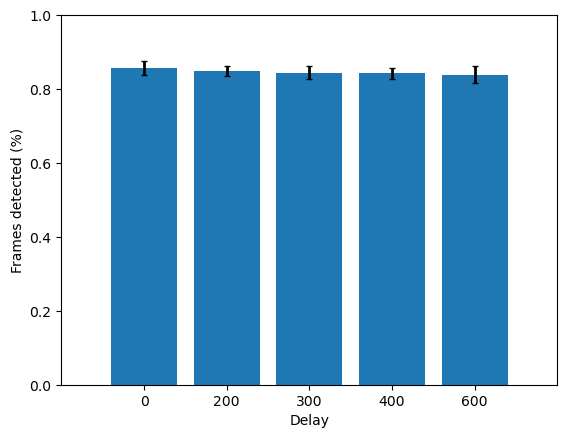
\includegraphics[scale=0.5]{images/frames-detected.png} 
   \caption{Form answers averaged for all subjects for each delay.}
   \label{fig:frames-detected}
\end{figure}

To make for better averages over different trials, all NaN values, i.e frames where no apriltag was detected in the frame, were linearly interpolated. To illustrate this one result is shown before and after interpolation in \ref{fig:raw-vs-interpolated}. 

\begin{figure}[!hbt]
   \centering
   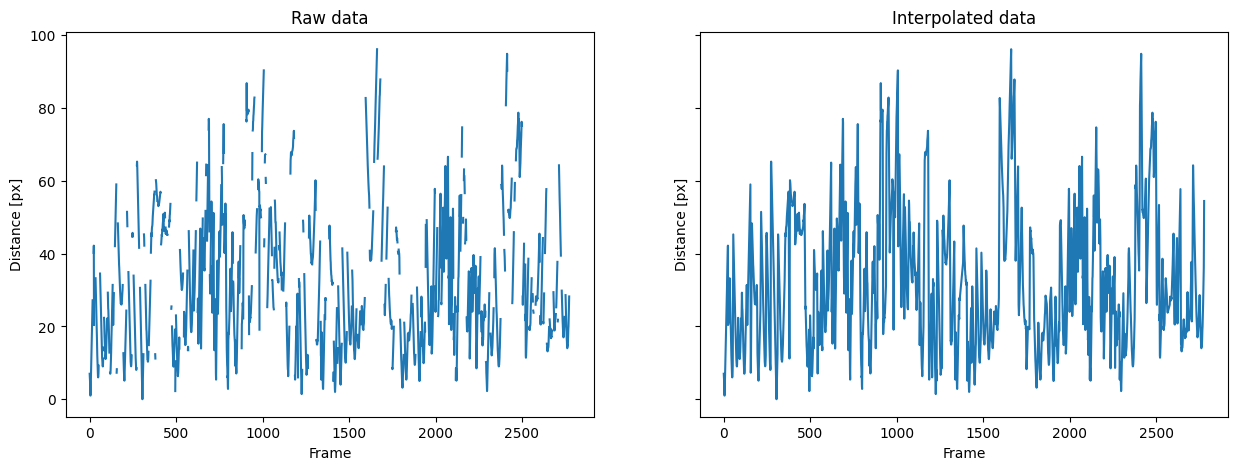
\includegraphics[scale=0.5]{images/raw-vs-interpolated.png} 
   \caption{Results for one trial: to the left the result with NaN-values and to the right interpolated result.}
   \label{fig:raw-vs-interpolated}
\end{figure}

\subsubsection{Difficulty of the task}
The center of the apriltag did not have a very clear center which could have made it difficult for the subject to complete the task. To remedy this, a printed apriltag where the center was marked out, but it could be that the subject had difficulty identifying the exact center during the trial.

\subsubsection{Control Choppiness}
\label{sec:control-choppiness}
The control of the gimbal is done through a command sent to the drone with two angles for pitch and yaw. The drone then moves the gimbal to the desired position. Although the angle was provided as a float, small increases in angle did not produce movement. This resulted in the control being somewhat choppy despite the continous feeling of the joystick. The choppiness was larger when looking farther away from the drone, as the ratio between the angle and the movement of the gimbal was larger. 

\section{Field testing}
This experiment aimed at running the gimbal interface on the real drone in-flight. The SSRS have a permit to operate drones beyond visual line of sight within a delimited area of the archipelago of Gothenburg. Because of this, the drone can be flown longer distances while all communication going over the mobile network. 

\subsection{Goals}
The main goals of the field testing were:
\begin{itemize}
   \item confirm that the gimbal control did not interfere with the flight control software
   \item evaluate suitability of the controls in a dynamic environment
   \item compare the manual controls to the already existing ROI-mode
\end{itemize} 

\subsection{Preparations}
For the experiment the gimbal control interface used earlier was modified in order to run with the software and video streaming configured on the actual drone. The video and recording component was entirely removed and the IP address which the program connected to was changed to that of the 4G modem. 
In order to compare the new controls to the already existing ROI-mode, a button on the controller was mapped to switch between joystick-mode and ROI-mode, using pre-programmed GPS-points for the drone to look at.

\subsection{Outdoor Conditions}
The weather was sunny with almost no clouds. The ground level wind was estimated to be around 5-9 m/s and the temperature was around 12 degrees Celsius.

\subsection{Procedure}
A flight plan of 17 waypoints and 2 loiter-waypoints was uploaded to the drone. The first and the last waypoints were close to the launch and the rest were placed on a route out in the archipelago. The drone was launched in manual mode and was circled around the operators to confirm that all the systems were working. The gimbal control software was also confirmed to be working during this phase, and the latency of the control was estimated to be between one and two seconds. 
The drone was then switched into auto mode and the flight plan was started.

\chapter{Results}
This chapter will go through the main findings of the experiments. The quantative measurements will first be presented followed by the results from the forms and interviews. Lastly, the results from the field testing will be presented.

\section{QoE Experiment}
In this section the quantative and qualitative results of the QoE experiment are presented and discussed. 

\subsection{Quantative measurements}
In \ref{tab:averages} the mean and standard deviation of the different delays are presented. The values are also visualized in plot \ref{fig:avg-std}. A clear trend can be seen where both the mean and standard deviation increase with the delay. An interesting feature of the data is that the mean after 400ms starts to increase at a non-linear rate, while the standard deviation has a more or less linear increase all throughout the added delays.

\begin{table}[ht]
   \centering
   \begin{tabular}{|c|c|c|}
   \hline
   \textbf{Delay} & \textbf{ Mean} & \textbf{Std. deviation} \\
   \hline
   0 & 29.804138 & 18.030196 \\ \hline
   200 & 35.234192 & 22.347311 \\ \hline
   300 & 41.538190 & 26.805780 \\ \hline
   400 & 46.048449 & 28.718249 \\ \hline
   600 & 61.811312 & 37.226394 \\ \hline
   \end{tabular}
   \caption{Table caption goes here.}
   \label{tab:averages}
\end{table}


\begin{figure}[!hbt]
   \centering
   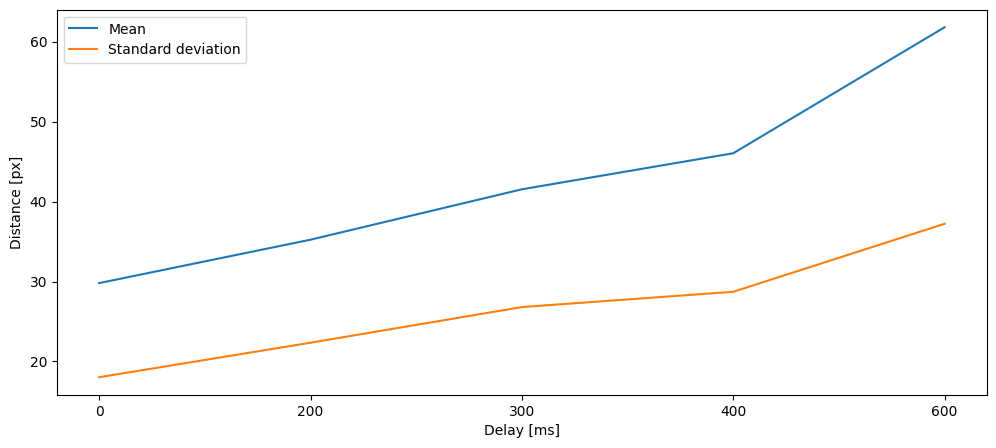
\includegraphics[scale=0.5]{images/avg-std.png} 
   \caption{Pixel error average and standard deviation for all delays. Delays 100 and 500 are added on the x-axis for correct scale.}
   \label{fig:avg-std}
\end{figure}

In figure \ref{fig:ecdf} the empirical cumulative distribution functions (ECDF) for the results of each delay are shown. The x-axis represents the value which the entry has while the y-axis represents the percentage of entries that are less than or equal to the x-axis value. The increase in both average and mean can be clearly observed as the delay increases. It can also be deduced that the distance between the center of the ECDF distributions for 0ms and 200ms is much smaller than that between the curves for 400ms and 600ms. This could indicate that the added 200ms added delay had a larger impact at 400ms than at 0 ms.

\begin{figure}[!hbt]
   \centering
   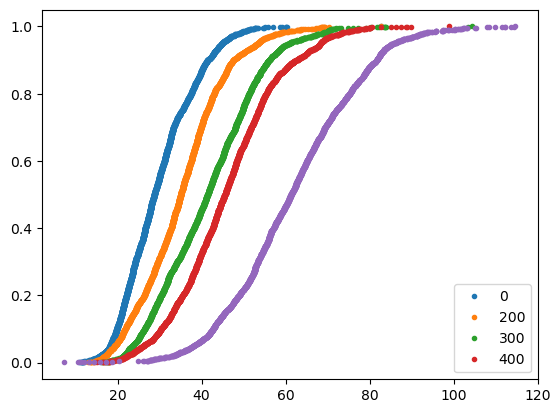
\includegraphics[scale=0.5]{images/ecdf.png} 
   \caption{ECDF of the total distance for all subjects. The curves show the distribution of the error for each delay. A larger inclination suggests a larger spread and the more to the right the curve is, the larger the average error.}
   \label{fig:ecdf}
\end{figure}

In figure \ref{fig:hoverboard-pos} all the values from the trials have been averaged and the position of the hoverboard has been superimposed. In this plot one can see that the final corner of the track is the most difficult, and that the very end and early beginning of the track are the easiest. 

\begin{figure}[!hbt]
   \centering
   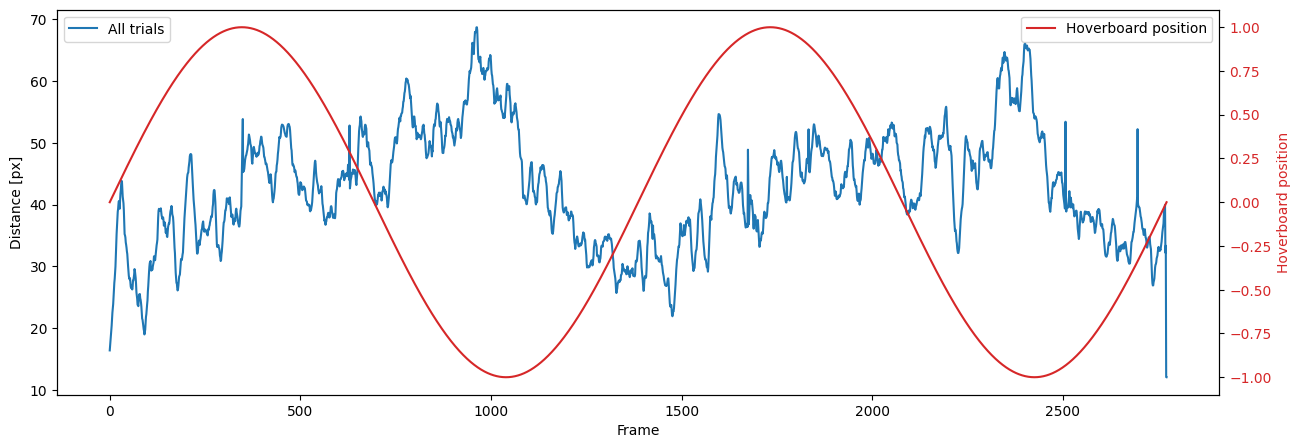
\includegraphics[scale=0.4]{images/hoverboard-pos.png} 
   \caption{All trials averaged with hoverboard position superimposed. The error steadily increases up until the end of the last corner where it decreases rapidly.}
   \label{fig:hoverboard-pos}
\end{figure}

To see the performance over the course of the hoverboard's track for each delay, the trials of all subjects were summarized on a particular delay alongside the position of the hoverboard. This is shown in \ref{fig:0vs600}, where all trials with 0ms and 600ms added delay are averaged on each frame. The more transparent blue and green lines represent the average over all trials while the darker lines are a rolling average of the data. The red line represent the position of the hoverboard.
It can be seen that there is a    

\begin{figure}[!hbt]
   \centering
   \makebox[\textwidth]{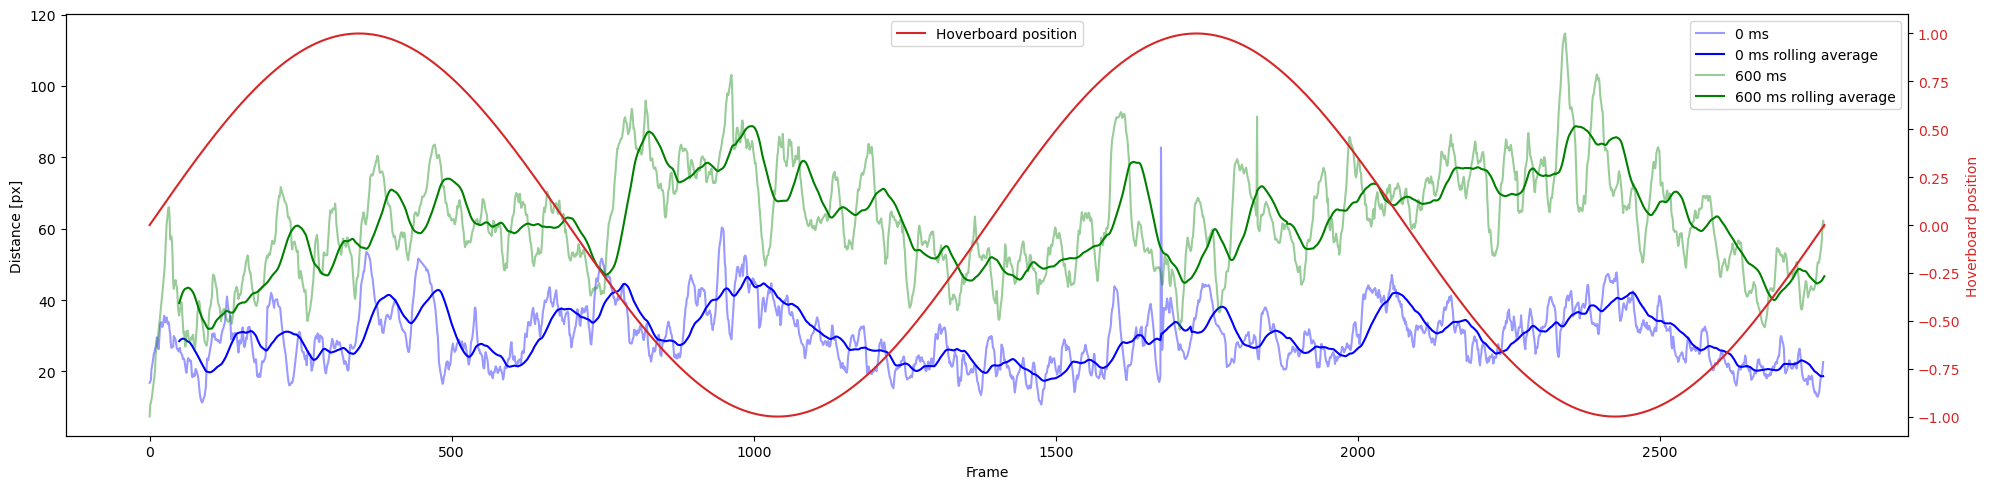
\includegraphics[scale=0.35]{images/0vs600.png}}
   \caption{Total trials for latencies 0 and 600 averaged over all subjects.}
   \label{fig:0vs600}
\end{figure}


\subsection{Forms and interviews}
In this section the results from the forms and interviews are presented and discussed.

\subsubsection{Trial forms}
In \ref{fig:form-ans} the answers from the questionnaires filled out after each trial are averaged over all subjects and visualized as a grouped bar chart. It is important to note that the jumps in delay are not uniform. The questions can be seen in \ref{tab:form-questions}. 

Here follows a brief analysis of the results for each question in \ref{fig:form-ans}
\begin{description}
   \item[1: Controllability] 
   The controllability decreases dramatically over all delays. Although the ratings decrease with added delay, the answers suggest that the sence of controllability did not differ much between 400ms and 600ms added delay, and that the answers could plateau with further added delay.  

   \item[2: Ability to perform task] 
   The average ratings for 200ms, 300ms, and 400ms are very similar. The added delay seems to have had little effect on the impression of their task performance, in spite of the quantative results showing a significant difference in pixel error. The subject's answer does however depend heavily the subject's interpretation of the task and how close is "good enough".
 
   \item[3: How pleasant was the system to use]
   The ratings of the pleasantness of the system seem to decrease steadily with added delay for each interval.

   \item[4: Impression of the system as a whole] 
   The system with 0ms added delay clearly made a better impression on the subjects. An interesting feature of the answers is that the systems with 200ms and 300ms have gotten the exact same rating.

\end{description}

\begin{figure}[!hbt]
   \centering
   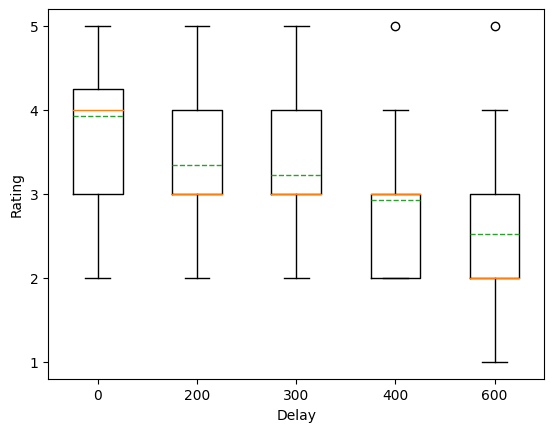
\includegraphics[scale=0.6]{images/form-ans.png} 
   \caption{Form answers averaged for all subjects for each delay.}
   \label{fig:form-ans}
\end{figure}

\subsubsection{SSQ}
In \ref{fig:ssq-ans} the difference in SSQ answers before and after the trials been averaged over all subjects. The largest response increase is on symptom four, namely "eye strain", which had an average increase of  0.5 with four out of all the subjects reporting an increase. The next two highest symptoms were "fullness of head" and "blurred vision". 

The results from the SSQ suggest a small increase in  symptoms after the trials, but the increase is not large enough to be considered significant for a sample size of only 10 subjects.

\begin{figure}[!hbt]
   \centering
   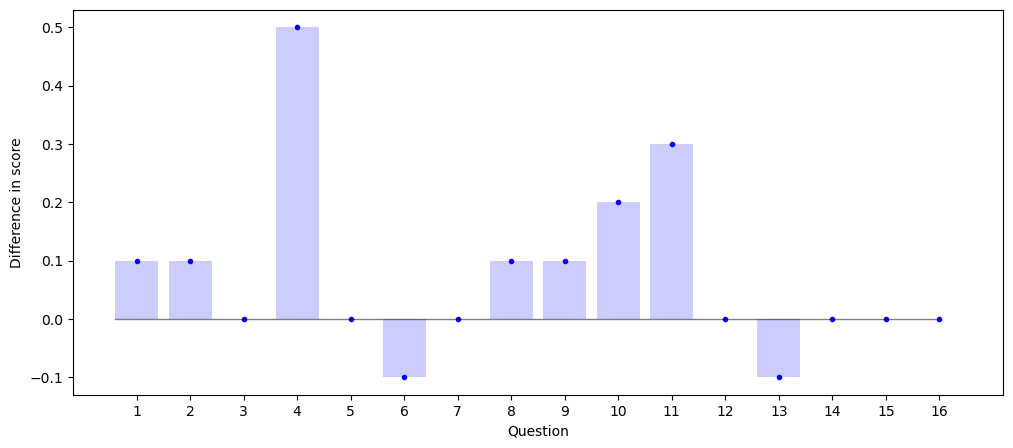
\includegraphics[scale=0.6]{images/ssq-results.png} 
   \caption{Difference in SSQ answers from before and after the trials on a scale from 0 to 4.}
   \label{fig:ssq-ans}
\end{figure}

\subsubsection{Interviews}
The answers to the interview questions will be summarized in this section.

\titleformat{\paragraph}[hang]{\normalfont\small\bfseries}{\theparagraph}{1em}{}
\titlespacing*{\paragraph}{0pt}{3.25ex plus 1ex minus .2ex}{1em}

\paragraph{1. What was your general experience of controlling the camera?}
A majority of the subjects reported that camera controls felt choppy, which is probably caused by the controls, explained in section \ref{sec:control-choppiness} on control choppiness. The subjects also reported that the controls felt very different throughout the trials. Some subjects also said that they grew more accustomed to the controls as the trials progressed.

Some quotes from the subjects are presented below.
\begin{description}
   \item[Subject 4545] "Had this been my day job I would have jumped out the window". 
   \item[Subject 1111] "Intuitive, sometimes there was delay that made it diffficult."
\end{description}

\paragraph{2. Did you experience any difference in the controls between the trials?}
All the subjects felt reported a difference in the trials. Usually subjects had a clear view on which trials were the easiest or the most difficult.

\paragraph{3. Was there any part of the track that was harder than any other?}
Almost all subjects reported that the last corner was the most difficult out of the entire track. This is supported by the quantative results as a visible spike in pixel error is present at that point in the track throughout all trials.
Some also stated that it was easier when the hoverboard was closer to the camera. This could be due to the effect of camera's choppiness which was less noticable short range, as explained in section \ref{sec:control-choppiness}.

\paragraph{4. Do you think the system would have been usable with the worst experimental conditions?}
On this question the answer of the subjects varied. A couple gave an absolute no, while others said that it depended on how exact one had to follow the object. 

\paragraph{5. Do you think training would have helped an operator get better using the system?}
All the subjects responded that training would improve one's performance in the system and that they got better at the task as the trials progressed. 

\section{Field Testing}
The gimbal control software integrated successfully into the running system and did not interfere with the controls during the course of the experiment. Thus, the first goal of the field testing was successfull. 
The two different modes of operation were tested and the results are presented in the following sections.

\section{Manual Control}
During the initial loiter, the plane's orientation changed quickly depending on where the plane was facing with respect to the direction of the wind. This made the gimbal very difficult to control manually, with the delay of the controls making it almost impossible to manually compensate with the joystick when the plane made an aggressive roll or yaw.

After the plane had left the initial loiters it had more time flying straight. During this time the camera was much easier to control manually, as the plane was more stable and the orientation was remained the same for an extended amount of time. 
Between the ?? and ?? waypoint, a boat was spotted slightly beside the plane. The gimbal operator decided to try and follow the boat. Although the delay made it more difficult to control the gimbal than in the lab experiment, the boat was successfully followed for a short time. An image from the video feed can be seen in figure ??. It was also observed that the position of the boat next to the aircraft could be estimated by the operator, allowing preemptive gimbal movements to compensate for the delay. 

Another observation from the experiment is that, being a fixed wing aircraft, the operator's ability to control the camera relies heavily on the manouvering of the aircraft, which means that improving the controls of the actual aircraft would improve the experience of controlling the camera significantly. 

\section{ROI Control}
The ROI-mode was activated on one of the loitering points and worked well when the perspective of the drone changed quickly. However, there were some inconsistencies in the altitude data for the points which caused the camera to point at a point below the surface of the earth. The point was adjusted by raising the altitude provided to the GPS-point. 

It could also be observed that increasing the loiter-radius gave a better image as the inexactness of the GPS-point was less impactful.

\chapter{Conclusion}
A test bed on the ArduPilot platform was successfully implemented and shown to work in a lab setting as well as in a real flight scenario. In the following sections the conclusions from the two experiments conducted with the test bed will be summarized.

\section{QoE Experiment}
From the quantative results a clear trend can be seen that the delay has a negative effect on the performance of the subjects. The task performance measure decreases linearly at first, but has a higher change rate for the 600ms added delay. Trials with higher added delays would have to be conducted to generalize the relationship between delay and task performance.

When taking into account the subject's rating of the system, it can be seen that the experience of a user is not always proportional to the worsening of QoS parameters. A slight increase in simulator sickness was observed, although it was not statistically significant.

\section{Field testing}
The results from the field testing shows that the gimbal software could be easily integrated with the system running on the real drone. The manual controls were also deemed suitable when the plane was flying in straight lines and when surveying or following an moving object compared to the already existing ROI-mode. When loitering the ROI-mode was found to be more practical.

\chapter{Future Work}
The test bed developed in the thesis work could be used for more experiments in a lab environment. It would be interesting to look at the effect of other delays as well as the effects of other network parameters such as jitter or image quality.
The modified test bed will(/can?) also be used as starting point for the gimbal control of the drone, and will help to evaluate the use case of drones for sea rescue further.


% Should use consistent formatting when it comes to Names ("FirstName LastName", or "F. LastName")
%\printbibliography
\makebibliography{MyMSc}

\end{document}